\documentclass[a4paper,12pt,twoside]{book}
\usepackage[english]{babel} 
%\usepackage[italian]{babel} 
%\usepackage[latin1]{inputenc} 
\usepackage[dvips]{graphicx}
\usepackage{amssymb}
\usepackage[width=125mm]{caption}
\usepackage{amsthm}
\usepackage[ND,SEQ]{prftree}
\usepackage{mathrsfs}
\usepackage{graphicx}
\usepackage{amsmath}
%\usepackage{bookman}


\usepackage{fancyhdr}
 
\pagestyle{fancy}
\fancyhf{}
%\fancyhead[LE,RO]{Share\LaTeX}
\fancyhead[CE]{\leftmark}
\fancyhead[CO]{\rightmark}
\fancyfoot[LE,RO]{\thepage} 
\renewcommand{\headrulewidth}{1pt}
%\renewcommand{\footrulewidth}{1pt}   %not visible if commented 

\usepackage[pdfauthor={Paolo Comensoli},
pdftitle={Hyper-resolution principle, applications to Nullstellensatz and graphs, 
Paolo Comensoli}, pagebackref=true]{hyperref}


% Dimensione della pagina
\setlength{\oddsidemargin}{.3in}  % Distance from the left edge -1 inch 
\setlength{\textwidth}{145mm}     % Normal width of the text
\setlength{\topmargin}{.25in}     % Distance from top to PAGE'S HEAD -1 inch
\setlength{\textheight}{225mm}    % Height of the body of page
\setlength{\headheight}{0mm}      % Height of a box containing the head
\setlength{\parskip}{0.5mm}       % Extra vertical space before a paragraph
\setlength{\parindent}{9mm}       % Width of the indentation 
\linespread{1.65}                 % Line spacing        

\newtheorem{theorem}{Theorem}[chapter]
\newtheorem{proposition}[theorem]{Proposition}
\newtheorem{definition}[theorem]{Definition}
\newtheorem{lemma}[theorem]{Lemma}
\newtheorem{corollary}[theorem]{Corollary}

\newcommand{\E}{\mathscr{E}}
\newcommand{\J}{\mathcal{J}}
\newcommand*{\QEDF}{\hfill\ensuremath{\blacksquare}}
\newcommand*{\QED}{\hfill\ensuremath{\square}}

\newcommand*\npred{\,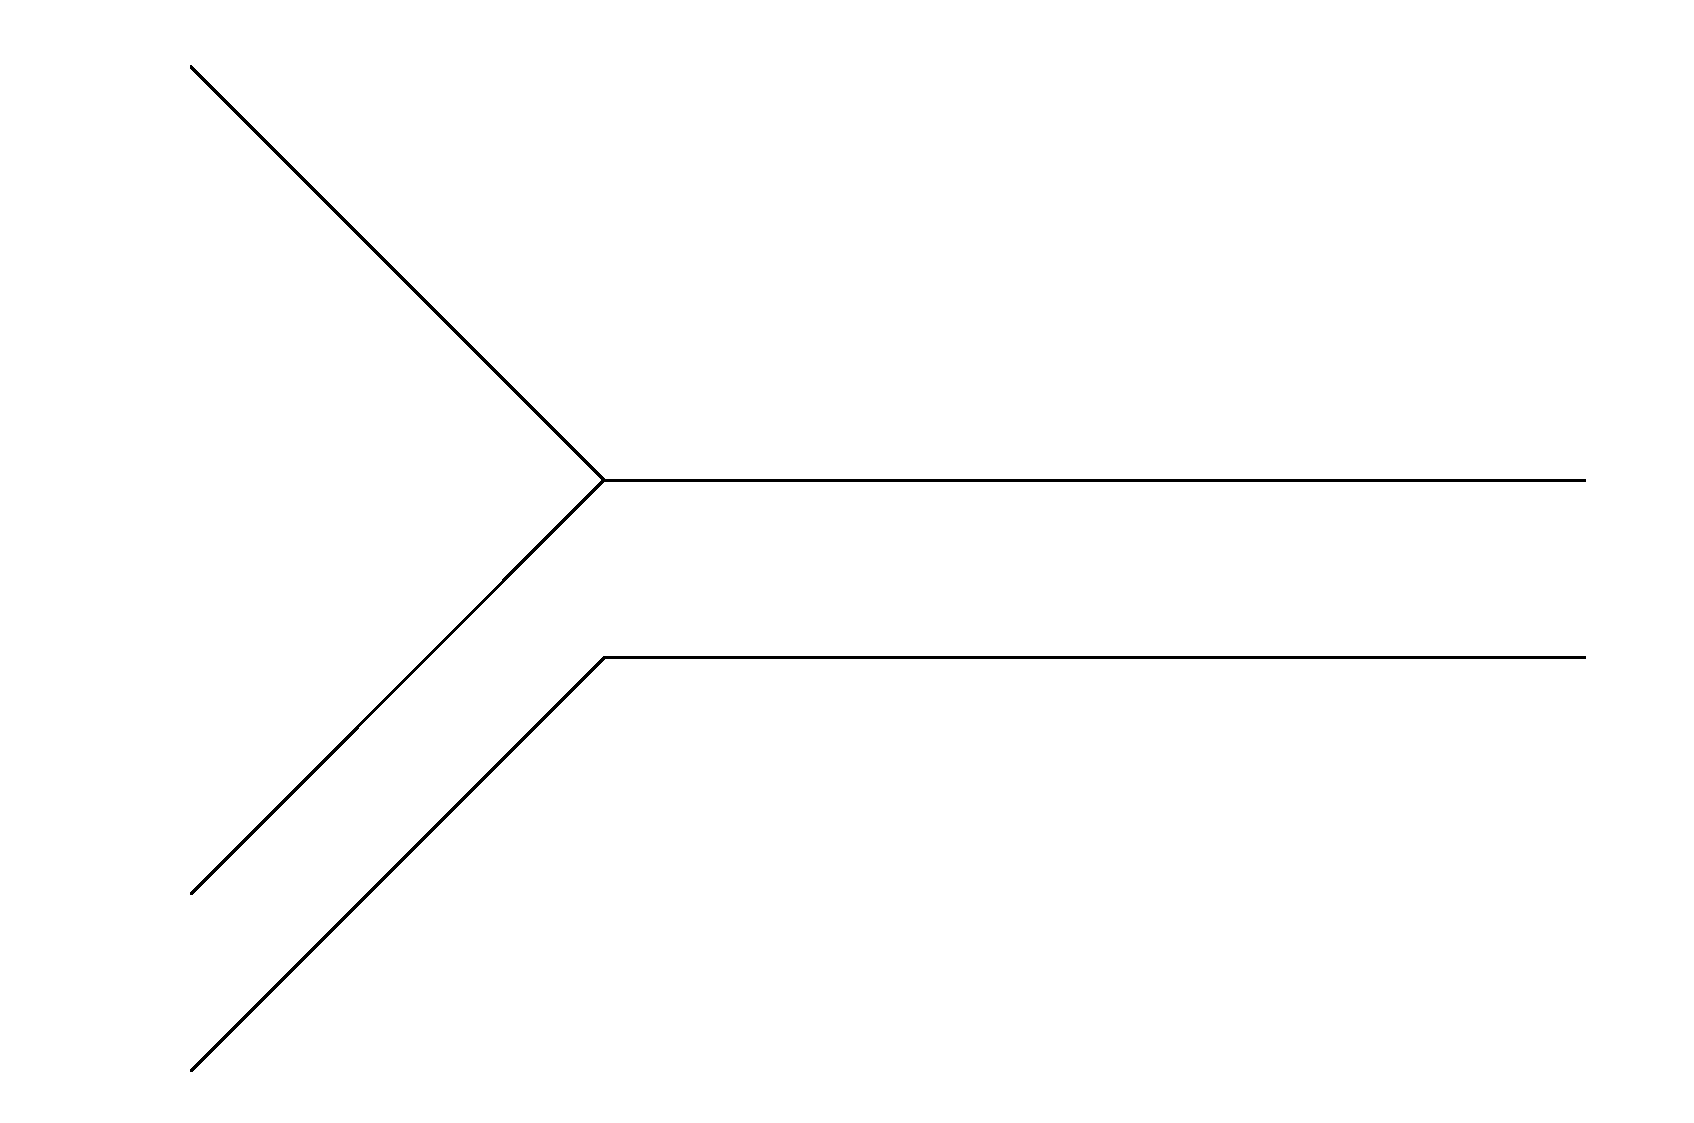
\includegraphics[scale=0.02]{./simboli/not-predecessor.eps}\,}
\newcommand*\pred{\,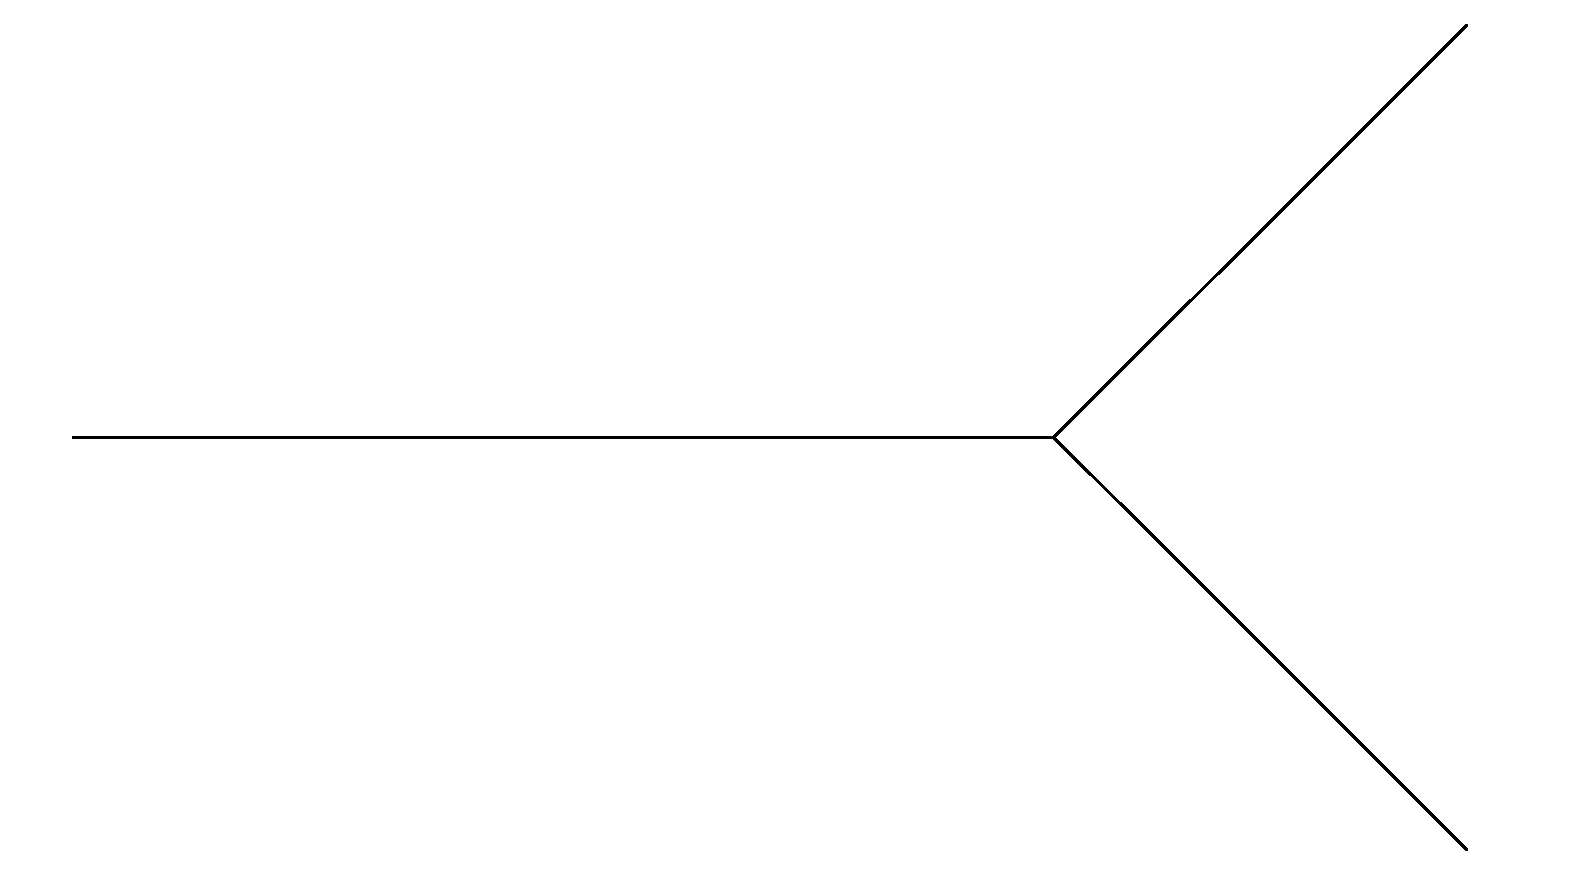
\includegraphics[scale=0.02]{./simboli/predecessor.eps}\,}

\let\oldemptyset\emptyset
\let\emptyset\varnothing
\let\o\vee
\let\e\wedge

\title{Hyper-resolution principle, applications to discrete mathematics}
\author{Paolo Comensoli}
\date{14/05/2018}

\begin{document}

\maketitle
\thispagestyle{empty}
\tableofcontents
\newpage
\subsection*{Introduction}

\thispagestyle{empty}
\noindent In the first two sections I will expand some details of the Lifschitz's work \cite{lifschitz}.
First of all I will briefly give the hyper-resolution principle and Robinson's theorem as stated by Lifschitz, then I will show the proof of Nullstellensatz with the aim to clarify every step.\\
\textbf{Notation:}
\begin{itemize}
\item \textit{Literal:} an atomic formula or a negation of an atomic formula.
\item \textit{Clause:} a finite set of literals.
\item if $\Gamma$ is a clause, $\overline{\Gamma}$ is the disjunction of the elements of $\Gamma$ in a fixed order.
\end{itemize}


\chapter{Hyper-resolution principle}

Let $T$ be a set of propositional formulae, each of the form:
$$\bigwedge_{i=1}^m A_i \rightarrow \bigvee_{j=1}^n B_j 
$$Where the $A_i$'s and $B_j$'s are literals and $m+n>0$.\\
We have the calculus $H_T$: the objects derivable are clauses and the rules of inference are:
\begin{equation}\label{axiom}
\prftree{\Gamma_1 \cup \{A_1\} ,} {\cdots,} {\Gamma_m \cup \{A_m\} } 
{\Gamma_1\cup\cdots\cup\Gamma_m\cup\{ B_1 ,\cdots ,B_n\}}
\end{equation}
for every element of $T$. The formulae of the set $T$ will be called the \textit{non-logical axioms} of $H_T$


\noindent\textbf{Example} Let $T=\{ A \rightarrow B \o C ,\; A,\; \neg B \}$, then $H_T$ has three rules:

\begin{center}
\begin{tabular}{ccc}
$$\prftree{\Gamma \cup \{A\} }  {\Gamma\cup \{B,C\}} 
$$
& \hspace{5mm}
$$\prftree{\Gamma }  {\Gamma\cup \{A\}} 
$$
& \hspace{5mm}
$$\prftree{\Gamma \cup \{B\} }  {\Gamma }
$$
\end{tabular}
\end{center}
Using such rules we get the tree:
$$
\prftree{\prftree{\emptyset}{\{A\}}}
{\prftree{\{B , C\}}{\{C\}}}
$$
and we write $\emptyset \vdash_{H_T} \{C\}$

Given a rule in the form (\ref{axiom}) and an application of it in a derivation, whenever $A_i \in \Gamma_i$ for some $i$, we call such application \textit{trivial}. The following two lemmas ensure that such kind of application can always be removed.

\begin{lemma}
Let $\Pi$ be obtained from $\Sigma_1,...,\Sigma_m$ by one application of a rule $H_T$. For any $\Sigma_1' \subset \Sigma_1,...,\Sigma_m' \subset \Sigma_m  $, one of the two following holds:\\
(a) $\Sigma_i' \subset \Pi$ for some $i$\\
(b) some $\Pi '\subset\Pi$ can be obtained from $\Sigma_1 ',...,\Sigma_m '$ by an application of the same rule
\end{lemma}

\emph{Proof:} Consider an application of (\ref{axiom}) leading from  $\Sigma_1,...,\Sigma_m$ to $\Pi$, for this application:
$$\Sigma_1=\Gamma_1\cup\{A_1\},...,\Gamma_m\cup\{A_m\}  $$
$$\Pi=\Gamma_1\cup ...\cup\Gamma_m\cup\{B_1,...,B_n\}$$
Consider the following two cases:\\
(a) $A_i \notin \Sigma_i '$ form some $i$. Then $\Sigma_i '\subset\Gamma_i\subset\Pi$
\\(b) $A_i \in \Sigma_i '$ for every $i$. Then $\Sigma_i '=\Gamma_i ' \cup \{A_i\}$ where $\Gamma_i '=\Sigma_i '\backslash \{A_i\}$, one application of (\ref{axiom}) to 
$\Sigma_1 ',...,\Sigma_m '$ gives 
$\Pi '=\Gamma_1 '\cup ...\cup\Gamma_m '\cup\{B_1,...,B_n\}\subset\Pi$

\begin{lemma}
For every derivation of a clause $\Pi$ in $H_T$ there exists a derivation of some $\Pi '\subset\Pi $ in $H_T$ without trivial application of rules of inference.
\end{lemma}

\begin{theorem}[\textbf{Robinson's, version 4}]
For any clauses $\Gamma_1, \cdots ,\Gamma_l , \Delta$, if in every model of $T$, the following is valid 
$$
\overline{\Gamma}_1\e\cdots\e\overline{\Gamma}_l \rightarrow \overline{\Delta}
$$
then there exists a derivation of some $\Delta' \subseteq \Delta$ from $\Gamma_1, \cdots ,\Gamma_l$ in $H_T$, containing no trivial application of rules of inference.
\end{theorem}


\chapter{Nullstellensatz}
Using Hyper-resolution principle and Robinson's theorem it is possible to prove the Nullstellensatz as stated here:

\noindent\textit{Let $K$ be a field and $f,f_1,\cdots, f_l \in K[\underline{x}]$, if in any extension of $K$, $f$ vanishes at all common zeros of $f_1,\cdots, f_l$, then there exists $p\in \mathbb{N}$ and $h_1,\cdots, h_l \in K[\underline{x}]$ such that} 
$$
f^p = \sum_{i=1}^l h_i \cdot f_i
$$
To this aim, consider the first order language $\mathscr{L}=\{+,\cdot,=\nobreak 0\}\cup\nobreak K$ where $+,\cdot$ are binary function symbols, $=0$ is a unary predicate symbol and the elements of $K$ are constants; so the terms are polynomials over $K$ and the atomic formulae are algebraic equations.

\noindent Consider the theory given by the following axioms:
\begin{eqnarray}
& 0=0  \label{ax00} \\
& \neg (1 =0) \\
& r_1=0 \rightarrow r_2 =0 \qquad (r_1,r_2 \texttt{ are equal polynomials}) \\
& ( r=0 \e s=0) \rightarrow r+s=0 \\
& r=0 \rightarrow r\cdot s=0 \\
& r\cdot s=0 \rightarrow (r=0 \o s=0) \label{axintdom}
\end{eqnarray}
One can prove the equality axioms, the axioms of integral domain and the diagram of $K$. It follows that the models of the theory are the integral domains that contains $K$. Lifschitz, instead of the axiom $\neg (1=0)$, uses the axioms  $\neg (\alpha =0)$ for each $\alpha\in K\setminus \{0\}$, however the one taken here is equivalent and simplifies the next arguments.  

The calculus $H_T$ consists of the axiom $\{0=0\}$ and of the rules of inference:

\begin{equation}\label{non1=0}
\prftree{\Gamma \cup \{1=0\}}{\Gamma}
\end{equation}

\begin{equation}\label{eqpoly}
\prftree{\Gamma \cup \{r_1=0\} } { \Gamma \cup \{r_2=0\} } \qquad r_1,r_2\texttt{ are equal polynomials}
\end{equation}

\begin{equation}\label{somm}
\prftree{\Gamma \cup \{r=0\},}{\Delta \cup \{s=0\}}{\Gamma \cup \Delta \cup \{r+s=0\} } 
\end{equation}

\begin{equation} \label{mol}
\prftree{\Gamma \cup \{r=0\}}{\Gamma \cup  \{r\cdot s=0\} } 
\end{equation}

\begin{equation} \label{intdom}
\prftree{\Gamma \cup \{r\cdot s=0\}}{\Gamma \cup  \{r=0,s=0\} } 
\end{equation}
Note that the rules (\ref{non1=0}-\ref{mol}) do not increase the number of elements of the clauses, precisely for an application 
$$
\prftree[r]{(\ref{non1=0}-\ref{mol}) } {\Gamma}{\Delta}{\hspace{2mm}\Sigma\hspace{2mm}}
$$
we have $ |\Sigma| \leq   |\Gamma\cup\Delta|$; while for rule (\ref{intdom})
we have $\Delta = \emptyset$ and  $ |\Sigma| =   |\Gamma| +1 $. \\

For any derivation in $H_T$ there is a tree with all the applications of the rule (\ref{intdom}) at the bottom; this is ensured by the following.
\begin{lemma}\textit{Every derivation in $H_T$ which contains non-trivial applications can be rearranged in such a way that any application of (\ref{intdom}) is either the last one or it is followed by an application of (\ref{intdom})}.
\end{lemma}
\emph{\noindent \textit{Proof: }}Suppose to have a non-trivial application of a rule (\ref{intdom}) followed by a rule ($x$) different from (\ref{intdom}):
$$
\prftree[r]{$x$}
{\prftree[r]{\ref{intdom}}
{\Gamma\cup\{r\cdot s=0 \}}
{\Gamma\cup\{r=0, s=0 \}\,,}
}
{\Delta}
{\hspace{7mm}\Sigma\cup\{r=0,s=0 \}\hspace{13mm}}
$$

\noindent Here $\Delta$ is the second premise in case ($x$) is the rule (\ref{somm}), otherwise it should be dropped. In the case that both $r=0$ and $s=0$ in the conclusion are different from $A_1$  shown in the scheme (\ref{axiom}) of the rule ($x$), then $A_1\in\Gamma$  and we can change the order as follow:

$$
\prftree[r]{\ref{intdom}}
{\prftree[r]{$x$}
{\Gamma\cup\{r\cdot s=0 \}, \hspace{7mm}}    {\Delta}
{\hspace{7mm}\Sigma\cup\{r\cdot s=0 \}\hspace{7mm}}}
{ {\Sigma\cup\{r=0, s=0 \}}} 
$$

Otherwise let $\{r=0\}$ be $A_1$ of ($x$), depending on whether ($x$) is (\ref{non1=0}),(\ref{eqpoly}) ,(\ref{somm}) or (\ref{mol}), change the derivation according to one of the schemes below


\begin{eqnarray*}
\prftree[r]{\ref{non1=0}} { \prftree[r]{\ref{intdom}} {\Gamma \cup  \{1\cdot s=0\}} {\Gamma \cup  \{1=0, s=0\}} } {\Gamma \cup \{s=0\}}
&  \leadsto 
 &\prftree[r]{\ref{eqpoly}} { \Gamma \cup \{1\cdot s=0\}   } {\Gamma \cup \{s=0\}}
\end{eqnarray*}



\begin{eqnarray*}
\prftree[r]{\ref{eqpoly}} { \prftree[r]{\ref{intdom}} {\Gamma \cup  \{r_1\cdot s=0\}} {\Gamma \cup  \{r_1=0, s=0\}} } {\Gamma \cup \{r_2=0, s=0\}}
&  \leadsto 
\prftree[r]{\ref{intdom}} { \prftree[r]{\ref{eqpoly}} {\Gamma \cup  \{r_1\cdot s=0\}} {\Gamma \cup  \{r_2\cdot s=0\}} } {\Gamma \cup \{r_2=0, s=0\}}
\end{eqnarray*}


\begin{eqnarray*}
\prfrulenameskip=0.4em\prflinepadbefore=1ex
\prftree[r]{\ref{somm}} { \prftree[r]{\ref{intdom}} { \Gamma \cup \{ r\cdot s=0\}} { \Gamma \cup \{ r=0,s=0\} }  }{ \Delta \cup \{t=0\} }
{\hspace{11mm}\Gamma \cup \Delta \cup\{r+t=0, s=0\}\hspace{11mm}}
& \leadsto
& \prftree[r]{\ref{intdom}} 
{\prftree[r]{\ref{eqpoly}}
{ 
\prftree[r]{\ref{somm}}{\Gamma \cup \{r\cdot s=0\},} 
{ \prftree[r]{\ref{mol}} {\Delta \cup \{t=0\}  }  {\Delta \cup \{t\cdot s=0\} }}
{\Gamma \cup \Delta \cup \{r\cdot s+t\cdot s=0\} }
}
{\Gamma \cup \Delta \cup \{(r+t)\cdot s=0\} }
}
{\Gamma \cup \Delta \cup\{r+t=0, s=0\}}
\end{eqnarray*}


\begin{eqnarray*}
\prftree[r]{\ref{mol}} { \prftree[r]{\ref{intdom}} {\Gamma \cup  \{r\cdot s=0\}} {\Gamma \cup  \{r=0, s=0\}} } {\Gamma \cup \{r\cdot t=0, s=0\}}
&  \leadsto 
\prftree[r]{\ref{intdom}} 
{ \prftree[r]{\ref{eqpoly}} 
{\prftree[r]{\ref{mol}}
{\Gamma \cup \{r\cdot s=0\}}
{\Gamma\cup\{ (r\cdot s) \cdot t \}} } 
{\Gamma \cup  \{(r\cdot t) \cdot s=0\}} } 
{\Gamma \cup \{r\cdot t=0, s=0\}}
\end{eqnarray*}
By a series of application of this procedure, we obtained a derivation as required. 

\QED

Now we have all the tools to achieve the proof of nullstellentsatz:
\\\textbf{\textit{Proof: }} Let $K$ be a field and $f,f_1 \cdots f_l \in K[\underline{x}] $  such that  in any extension of $K$, $f$ vanishes at all common zeros of $f_1\cdots f_l$. 
This amounts to require that in every model of (\ref{ax00}-\ref{axintdom}) the following is valid:
$$ \Gamma_1\e\cdots\e\Gamma_l\rightarrow\Delta$$
where $\Gamma_i=\{f_i=0\}$ and $\Delta =\{f=0\}$.\\ Then by Robinson's theorem: $\Gamma_1,\cdots ,\Gamma_l \vdash_{H_T} \Delta '$ where either $\Delta '=\emptyset$ or $\Delta '=\{f=0\}$. 
In particular take a derivation without trivial applications and where all the applications of (\ref{intdom}) are at the bottom, the existence of such tree is ensured by the lemma shown above. The tree is of the form:
\begin{equation}
\prfsummary[only rules \ref{intdom}] {\prftree[r]{\ref{non1=0}-\ref{mol}}{\Gamma_1,}{...,}{\Gamma_l}{\Sigma}}{\Delta '}
\end{equation}
Since all the $\Gamma_i$'s are singletons, and since the rules (\ref{non1=0}-\ref{mol}) do not increase the size of the clauses, $\Sigma$ is either a singleton or the empty set. Let's treat separately the cases of $\Delta '$.

\textbf{\emph{Case $\Delta '=\emptyset$}} \\
The only way to get $\emptyset$ out of the rules of inference is by applying (\ref{non1=0}), in this case rule (\ref{intdom}) does not apply at all and the tree is of the form: 
$$
\prftree[r]{\ref{non1=0}}
{ \prftree[r]{\ref{eqpoly} - \ref{mol}}
{ \Gamma_1, }{\cdots ,}{\Gamma_l}
{\hspace{5mm}\{1=0\}\hspace{5mm}	} 
}
{\emptyset }
$$
1 is obtained by a series of applications of rules (\ref{eqpoly} - \ref{mol}), therefore it is a linear  combination of $f_1,\cdots ,f_l\;$ : 
$$f^0=1 = \sum_{i=1}^l h_i \cdot f_i$$


\textbf{\emph{Case $\Delta '=\{f=0\}$ }} \\
Suppose that rule (\ref{intdom}) applies $p-1$ times, (\ref{non1=0}) does not apply at all and the tree is of the form:
$$
\prftree[r]{$(p-1)$ applications of \ref{intdom}}
{ \prftree[r]{\ref{eqpoly} - \ref{mol}}
{ \Gamma_1, }{\cdots ,}{\Gamma_l}
{\hspace{7mm}\Sigma\hspace{7mm}	} 
}
{\{f=0\} }
$$
Since (\ref{intdom}) applies and $\Sigma$ is a singleton, $\Sigma$ must be of the form $ \{ t_1 \cdot r_1 =0 \}$. Suppose that the $A_1$ of the $i^{th}$ application is $r_i=t_{i+1}\cdot r_{i+1}$, then the tree is:
$$
\prfsummary{
\prftree[r]{ \ref{intdom}}
{ \prftree[r]{\ref{eqpoly} - \ref{mol}}
{ \Gamma_1, }{\cdots ,}{\Gamma_l}
{\hspace{7mm}\{t_1 \cdot r_1=0\}\hspace{7mm}	} 
}
{\{ t_1=0, t_2 \cdot r_2=0\} }
}
{\prftree[r]{\ref{intdom}}
{\{ t_1=0,\cdots t_{p-2}=0, t_{p-1}\cdot r_{p-1}=0\}  }
{\{ t_1=0,\cdots ,t_{p-1}=0,r_{p-1}=0\}}
}
$$
Since the root of the tree must be the singleton $\Delta '=\{f=0\}$, it is the case that for any $i$: $t_i=r_{p-1}=f $.
Therefore $\Sigma= \{ f^p =0 \}$ and we conclude 
$$f^p = \sum_{i=1}^l h_i \cdot f_i $$


\QED
%
%\newpage
%$$
%\prftree[r,l]{$\o^-$}{yay $\quad$}
%{\prftree[r]{$\rightarrow^-$}{A}{A \rightarrow B\o C}{B\o C} }
%{\prfboundedassumption{C}}
%{\prftree[r]{$\rightarrow^-$}{\prftree[r]{$\rightarrow^-$}{\prfboundedassumption{B}}{\neg B}{\bot}}{ \prfsummary{EFQ}{\bot \rightarrow C}}{C} }
%{C}
%$$
%
%
%
%
%
%$$\prftree[r]{$\scriptstyle\supset\mathrm{I}$}
%{\prftree[r]{$\scriptstyle\supset\mathrm{I}$}
%{\prftree[r]{$\scriptstyle\supset\mathrm{E}$}
%{\prfboundedassumption{A}}
%{\prfboundedassumption{\neg A}}
%{\bot}}
%{\neg\neg A}}
%{A \supset \neg\neg A}
%$$



\chapter{Applications to graph theory}
In this chapter I will discuss applications of the resolution principle to graph theory, in particular we will face two different and equivalent ways of describing $n$-colourable graphs via resolution. The first approach relies on propositions of the kind "the vertex $x$ has the same colour of the vertex $y$", this method will be used to give a constructive proof that a graph is 2-colourable if and only if it does not contain odd cycles. The second approach assigns to each colour a number and relies on proposition of the kind "the vertex $x$ has a colour number smaller than the one of $y$", in other words this method introduces a partial order on the vertices and therefore it will introduce a stronger transitivity rule; this method will be used to prove Gallai-Hasse-Roy-Vitaver theorem, which gives a characterization of the chromatic number of a simple graph, by describing a partial order among vertices using directed paths and retrieving the $n$-colurable property by showing that such order can be used also for colours. Finally I will show another characterization of the chromatic number which generalizes the characterization of bipartite graphs and that may be used to state the four colour theorem.


\newpage
\section{Recalls of graph theory}
In this section I will briefly recall some notions of graph theory, for the part on simple graphs I will adopt the notation and terminology of Diestel \cite{diestel}, while for directed graphs I will mainly refer to Chartrand-Zhang \cite{chrom}. Some of the result shown here will be also shown in the next section using resolution methods, it might be interesting to compare the proofs and how different they are.

A simple graph $G$ is a couple of sets $(V,E)$ such that the elements of $E$ are unordered couples of elements of $V$. The elements of $V$ are called \textit{vertices} and the elements of $E$ are called \textit{edges}. A vertex $v$ is \textit{incident} with an edge $e$ if $v$ is one of the two elements of $e$, the two vertices incidents an edge are called its \textit{ends} and are said to be \textit{adjacent}; an edge whose endpoints are $x$ and $y$ is denoted as $xy$. 
A graph $G'=(V',E')$ is a \textit{subgraph} of G if $V' \subseteq V$ and $E' \subseteq E$.

A \textit{path} is a graph $P=(V,E)$ of the form:
$$ V=\{x_0,x_1, ..., x_n\} \qquad E=\{x_0 x_1, x_1x_2,.. x_{n-1}x_n\}$$ 
where the vertices are pairwise different, the length of the path is defined as the cardinality of $E$ which is $n$; we often refer to a path by the natural sequence of the vertices, writing $P=x_0x_1...x_n$. A graph is \textit{connected} if for any two distinct vertices, there is a path between them.  
A \textit{cycle} is a path where $x_n$ coincides with $x_0$; a cycle of length $n$ will be briefly called n-cycle; if a n-cycle is a subgraph of $G$, we say that $G$ has a n-cycle. 

\noindent A connected graph which has no cycle is called \textit{tree}, trees are characterized by the following theorem
\newpage
\begin{theorem}[characterization of trees] The following are equivalent:
\begin{itemize}
\item[(1)] $T$ is a tree
\item[(2)] for any edge $e$ of $T$, $T-e$ is not connected   
\item[(3)] any two vertices of $T$ are linked by a unique path
\item[(4)] $T$ is maximally acyclic, i.e. for any two vertices $u,v$ such that $uv$ is not an edge of $T$, $T+uv$ has a cycle
\end{itemize}
\end{theorem}
\noindent\textit{Proof}: 

(1)$\Rightarrow$(2):\\
If $uv$ is an edge of $T$ such that $T-uv$ is still connected, there is a path from $u$ to $v$ that does not pass trough the edge $uv$, such path concatenated with $uv$ makes a cycle in $T$.

(2)$\Rightarrow$(3):\\
If there are two distinct vertices $u,v$ of $T$ which are linked by two different  path, there is an edge $e$ which does not belong to both paths, then $T-e$ is still connected.

(3)$\Rightarrow$(1):\\
If it is connected and there is a cycle, for any two distinct vertices of the cycle there at least two path linking them.

(4)$\Rightarrow$(1):\\
If it's maximally acyclic it is also connected, indeed if the vertices $u,v$ are not linked by a path, $T+uv$ would be an acyclic graph and $T$ not maximally acyclic. 

(3)$\Rightarrow$(4):\\
Let $u,v$ be two distinct vertices of $T$, such that $uv$ is not an edge of $T$, if $u,v$ are connected by a path, there is a cycle in $T+uv$, hence $T$ is maximally acyclic.

\QED
\newpage For any connected graph $G$, it is always possible to obtain a tree by only removing edges, this tree is called \textit{spanning tree} and its existence is ensured by the following constructive proof.
\begin{proposition}[Spanning Tree]
Let $G=(V,E)$ be a connected graph, then there is a tree $T=(V,E')$ such that $E'\subseteq E$
\end{proposition}
\noindent\textit{Proof:}
Consider the following procedure: If $G$ has no cycle than it is a tree and we have obtained what we were seeking; otherwise let $e$ be an edge of $G$ that belongs to a cycle, then $G-e$ is still connected and we restart the procedure with $G-e$.
The algorithm always ends since $E$ is a finite set and it returns the required tree.\QED


A \textit{k-colouring} of a graph $G=(V,E)$ is a map $c:V \rightarrow \{1,..,k\} $ such that $c(v) \neq c(w) $ whenever $v$ and $w$ are adjacent; a graph is \textit{k-colourable} if it admits a k-colouring. The minimum positive integer $k$ such that $G$ is $k-$colurable is the \textit{chromatic number} and is denoted by $\chi (G)$.

A graph $G=(V,E)$ is bipartite if $V$ admits a partition in two subsets such that every edge has its ends in different subsets; clearly a graph is bipartite if and only if it is 2-colourable since we can assign a colour to each partition to obtain a 2-colouring and conversely whenever we have a 2-colouring we immediately obtain the partitions dividing vertices according to their colour. 
\begin{figure} 
\begin{center}
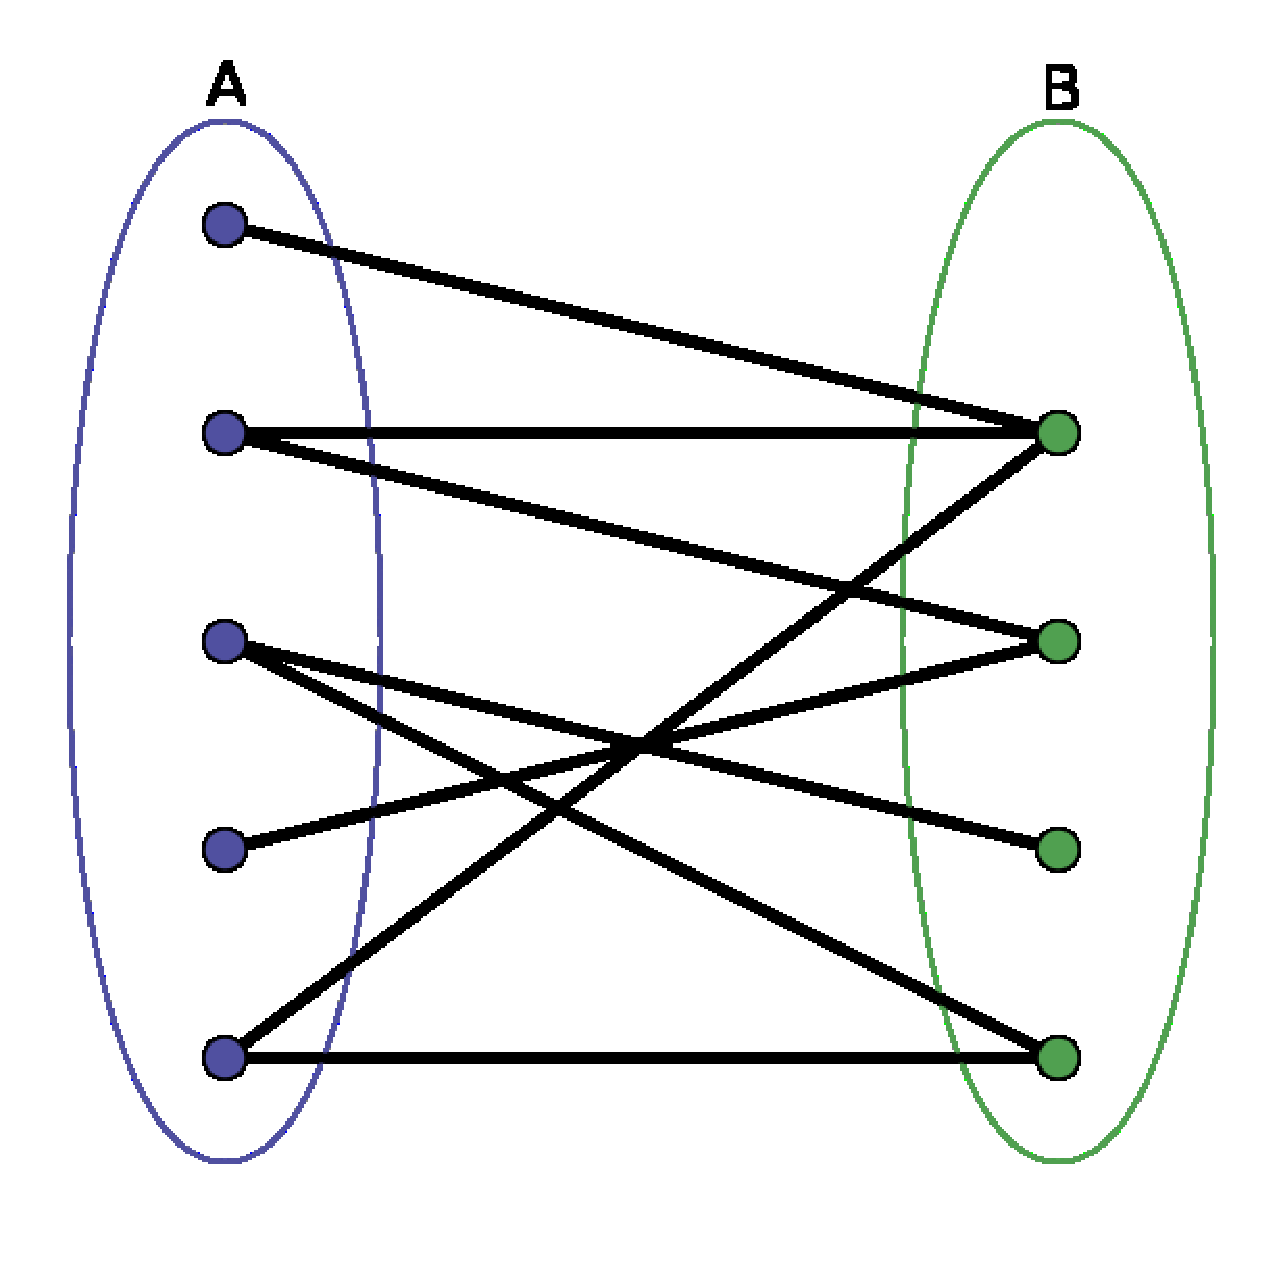
\includegraphics[scale=0.3]{bipartite.eps}
\caption{A bipartite graph coloured with two colours}\label{bip}
\end{center}
\end{figure}

Another important characterization of bipartite graph is the property of not having cycles of odd length.
\begin{theorem}
A graph $G=(V,E)$ is bipartite if and only if it does not contain odd cycles.
\end{theorem}
\textit{Proof:}
Suppose first that $G$ is bipartite; then $V$ can be partitioned into sets $U$ and $W$, so every edge has an end in $U$ and the other in $W$. Let $C=v_1v_2...v_nv_1$ be a $n-$cycle of $G$, if we assume $v_1\in U$, then $v_2\in W$, $v_3\in U$ and so on.
In particular $v_i\in U $ when $i$ is odd and $v_i\in W$ when $i$ is even, since $v_1\in U$ it follows $v_n\in W$ and $n$ is even.

Conversely, let $G$ be a graph without odd cycles. A graph is bipartite if all its components are bipartite, so assume the $G$ is connected. Let $T=(V,E')$ be a spanning tree of $G$ and fix a vertex $r\in V$, for any $v\in V$ let $d(v)$ be the length of the unique path from $r$ to $v$; now build the partitions $U,W$ of $V$ according to the following rule:
\begin{itemize}
\item if $d(v)$ is odd, $v\in U$
\item if $d(v)$ is even, $v\in W$
\end{itemize} 
Clearly $U\cap W =\emptyset$ and $U\cup W=V$, it remains to show that any $e\in E$ has its ends in different partitions. 
Let $xy\in E$, if it is the case that $xy\in E'$ then $d(x)=d(y)\pm 1$ and therefore they belong to different partitions. If $xy\notin E'$, then adding it to the spanning tree creates a cycle $C$ which is even since it is also e cycle of $G$; thus $C-xy$ is the unique path in $T$ from $x$ to $y$ and is of odd length, whence $d(x)$ and $d(y)$ have different parity.\QED

\subsection*{Directed graphs}
\addcontentsline{toc}{subsection}{Directed graphs}

A \textit{digraph} (or directed graph) $D$  is a couple of sets $(V,A)$ where the elements of $A$ are ordered couples of $V$. Elements of $V$ are still called vertices while elements of $E$ are called \textit{arcs} or \textit{directed edges}. For instance a representation of the digraph $D=(\{x,y,z\}, \{(x,y),(y,x),(x,z),(z,y)\})$ is shown in fig. \ref{digraph}

If for each pair of distinct vertices $u,v$ of a digraph $D$, at most one of $(u,v)$ and $(v,u)$ is an arc, $D$ is an \textit{oriented graph}. In fig. \ref{digraph} $D$ is not an oriented graph while $D_1$ and $D_2$ are good examples. Thus an oriented graph can be obtained from a simple graph $G$ by assigning a direction to each one of its edges, the digraph obtained in this way is said to be an \textit{orientation} of $G$; on the other hand starting from an oriented graph $D$ we obtain the \textit{underlying graph } by replacing all arcs $(u,v)$ with an edge $uv$. 

\begin{figure}[h]
\centering
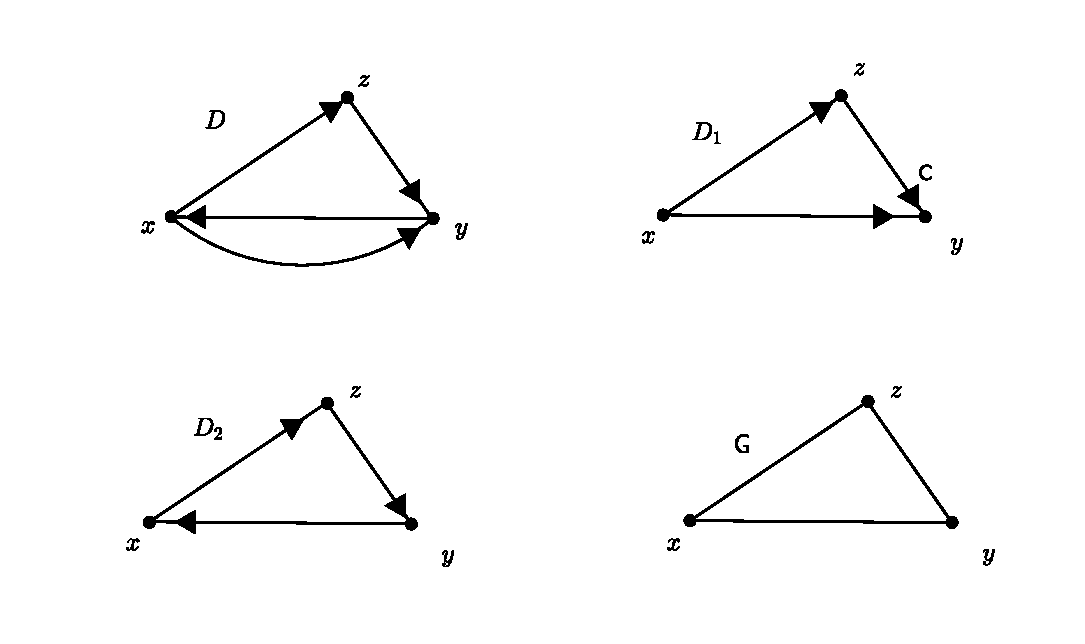
\includegraphics[scale=0.7]{digraphs.eps}
\caption{$D$ is a generic digraph;
		$D_1$ is an acyclic oriented graph;
		$D_2$ is a directed cycle;
		$G$ is the underlying graph of $D,D_1,D_2$}\label{digraph}
\end{figure}

\newpage
A sequence $x_0,...,x_n$ of distinct vertices of a digraph $D$ is a \textit{(directed) path} if for any $i$ $(x_i,x_{i+1})$ is an arc of $D$; a path in which $x_n$ coincides with $x_0$ and is called \textit{direct cycle}. Note that Fig. \ref{digraph} shows that an acyclic oriented graph may have an underlying graph with a cycle. As simple graphs have spanning trees and they are easy to obtain, digraphs have spanning acyclic digraph, they also have a maximality property, i.e. whichever arc is added, it creates a directed cycle.

\begin{lemma}[\textbf{Spanning acyclic digraph}]
Let $D=(V,A)$ be a connected digraph, then there is an acyclic oriented cycle $T$ which is connected and obtained by $D$ only by removing arcs.
\end{lemma}

The orientations of a simple graph can be useful to find the chromatic number, a characterization of $\chi (G)$ was found independently by L.M. Vitaver \cite{vitaver}(1962), M. Hasse \cite{hasse}(1963), B. Roy \cite{roy}(1967), T. Gallai \cite{gallai}(1969); here I will show the proof given by Chartrand and Zhang in their book \cite{chrom}, and later I will show the method adopted by Matijasevi\v{c} \cite{mat-1} which uses hyper-resolution.

Given a simple graph $G$ and an orientation $D$ of $G$, we define $\ell(D)$ as the length of the longest directed path in $D$. 
\begin{proposition}\label{prop-vitaver-easy}
There is an orientation $D$ of $G=(V,E)$ such that $$ \chi (G) \geq 1+\ell(D) $$
\end{proposition}   
We take a colouring map $c:V\rightarrow \{1,...,\chi (G)\}$, we build an orientation
 $D$ choosing a direction for each edge $uv$ of $G$, in particular we pick the arc 
 $(u,v)$ if $c(u)< c(v)$. In such orientation, any path is long at most $\chi 
 (G)-1$ whence $\ell(D)\leq \chi (G)-1  $, that is $ \chi (G) \geq 1+\ell(D) $ 
 
 \QED
\newpage
\begin{theorem}[The Gallai-Hasse-Roy-Vitaver theorem]\label{vitaver}
For every orientation $D$ of a graph $G=(V,E)$ $$\chi (G)\leq 1 + \ell(D)$$
\end{theorem}
Let $D$ be an orientation of $G$ and $D'$ a spanning acyclic subdigraph of $D$, we define a colouring map $c$ on $G$ by assigning to each vertex $v$ the colour 1 plus the length of the longest directed path of $D'$ that ends in $v$. Clearly the number of colours used is $1+\ell(D)$, indeed the longest path of $D'$ is also in $D$, otherwise $D'$ would not be maximal. 

Thus it remains to show that $c$ is a proper colouring, i.e. that if $uv\in E$, $c(u)\neq c(v) $, to this aim consider an arc $(u,v)$ of $D$, if it is also an arc of $D'$ then $c(u)<c(v)$; otherwise if it is not in $D'$, adding it creates a directed cycle which is the case only if there is a path from $v$ to $u$, thus $c(v)<c(u)$ 

\QED

\noindent The following result characterizes the chromatic number of a simple graphs and is a direct consequence of the last propositions.
\begin{corollary}\label{cor-vitaver}
Let $G$ be a graph and $\ell$ the minimum possible value of $\ell(D)$, $D$ orientation of $G$, then   
$$\chi (G)=1+\ell$$
\end{corollary}

\noindent\textit{Proof:}\\
Let $D$ be an orientation of $G$ such that 
$$\ell(D)=\ell=\textrm{min}\{\ell(D') \; 	,D' \textrm{ orientation of } G\}$$ 
then by Theorem \ref{vitaver} $\chi(G) \leq 1+\ell$. On the other hand by Proposition \ref{prop-vitaver-easy} for some orientatin $D'$  of $G$, $\chi(G)\geq 1+\ell(D')$; therefore, since $\ell(D')\geq\ell$ 
$$\chi (G)=1+\ell$$ \QED

\newpage 
The figure \ref{fig-vitaver} displays hot the Gallai-Hasse-Roy-Vitaver theorem applies to a cycle of length five, there are shown four different orientations of the cycle and to each vertex is assigned a colour based on how long is the longest directed path that reaches it. The rightmost orientation is not acyclic, every vertex is reached by a directed path of length five and they would all receive the same colour. The leftmost orientation is one that achieves the minimum $\ell(D)$ which in the case of odd cycles is 2, indeed the chromatic number for odd cycles is 3
\vspace{2cm}
\begin{figure}[h]
\centering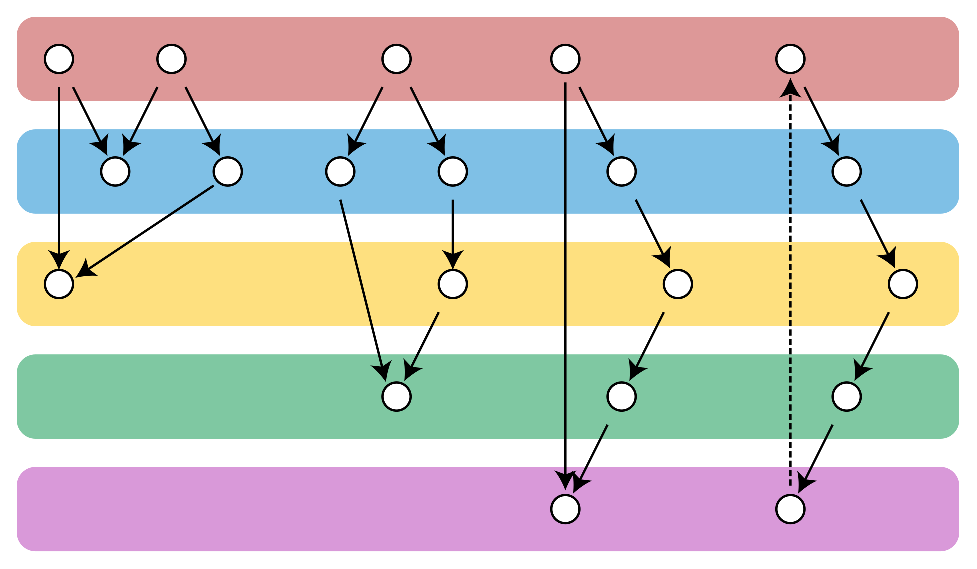
\includegraphics[scale=0.7]{vitaver.eps}
\caption{ }\label{fig-vitaver}
\end{figure}

\newpage
\section{Resolution approach to colouring}
Every colouring can be uniquely described (up to renaming the colours) by the symmetric binary relation "vertices $x$ and $y$ have the same colour", which we denote by  $\E xy$. 
Such binary relation, in order to represent a colouring map, should respect a transitivity axiom, and be false whenever the two vertices are adjacent 
\begin{gather}
\E xy \wedge \E yz \rightarrow  \E xz \label{color-prop1}\\
( xy \in E \Rightarrow ) \qquad  \neg \E xy \label{color-prop2}
\end{gather}
Also for an $n$-colouring we require that whenever we pick $n+1$ vertices at least 2 of them must share the colour, which amount to require for any $\{ x_0, x_1, ... , x_n \} \subseteq  V$
\begin{equation} \label{color-prop3}
\bigvee_{i=0}^{n-1} \bigvee_{j=i+1}^{n} \E x_i x_j
\end{equation}
Conversely if a binary symbol satisfies the above axioms, then it corresponds to some colouring map. More formally, for every graph $G=(V,E)$, we consider a language $\mathscr{L}=\{\E\}\cup V\cup E$, where $\E$ is a binary relation symbols and $V\cup E$ are constants; the models of the formulae (\ref{color-prop1}-\ref{color-prop3}) are the $n$-colourable graphs that contain $G$, if $G$ is not $n$-colurable the axioms are inconsistent and there are no models. The formulae (\ref{color-prop1}-\ref{color-prop3}) give rise to the calculus $H_G$ which consists of the following inference rules:
\begin{equation}
\label{trans}
 \prftree{\Gamma \cup \{\E xy \}}{\Delta \cup \{\E yz \}}{\Gamma \cup \Delta \cup \{\E xz \}}
\end{equation}
\begin{equation}
\label{jred}
\prftree[r]{$\quad xy \in E $}{\Gamma \cup \{\E xy \}}{ \Gamma}
\end{equation}
\begin{equation}
 \label{ax-col}
\prftree{\Gamma}{ \Gamma \cup \{\E x_0 x_1 , ... , \E x_{n-1} x_n  \}}
\end{equation}
Note that any tree made with these rules have (\ref{ax-col}) as leaves; on the other hand, if there are no trivial applications, rule (\ref{ax-col}) appears only at leaves, indeed $\emptyset\in\Gamma$ for every non-empty $\Gamma$.  \\
Besides axioms (\ref{color-prop1}), (\ref{color-prop2}), (\ref{color-prop3}) it should be necessary to add the axiom $\E xx$, I preferred to keep it implicit in the definition of the proposition symbol $\E$ in order to keep the formalism slightly lighter.

\subsection*{Bipartite graphs}
\addcontentsline{toc}{subsection}{Bipartite graphs}

\begin{proposition}
A graph $G=(V,E)$ that contains an odd cycle is not 2-colourable 
\end{proposition}
I will show that if there is an odd cycle the empty clause is derivable in $H_G$, i.e. $\vdash_{H_G} \emptyset$, and that therefore the propositions 	(\ref{color-prop1}-\ref{color-prop3}) are inconsistent.\\
Let $\{x_1, ..., x_{2n+1}\} $ be an odd cycle, by definition for $i=1,2,..., 2n$ $x_i x_{i+1} \in E$ and $ x_{2n+1} x_1 \in E$. Then consider the following deduction in $H_G$:
$$\prftree[r]{(\ref{trans})}
{
\prfsummary{ 
\prftree[r]{(\ref{trans})}
{\prftree[r]{(\ref{jred})}{
\prftree {\E x_1 x_2 , \E x_2 x_3 , \E x_1 x_3 }
{\E x_2 x_3 , \E x_1 x_3  }
}
{\E x_1 x_3}}
{ \prftree[r]{(\ref{jred})}
{ \prftree{ \E x_3 x_5 , \E x_4 x_5 , \E x_3 x_5}
{\E x_4 x_5 , \E x_3 x_5}
}
{\E x_3 x_5}}
{\E x_1 x_5}
}
{\E x_1 x_{2n-1}}
}
{
\prftree[r]{(\ref{jred})}{ \prftree{\E x_{2n-1} x_{2n},\E x_{2n} x_{2n+1},\E x_{2n-1} x_{2n+1} }{\E x_{2n} x_{2n+1},\E x_{2n-1} x_{2n+1}} }
{\E x_{2n-1} x_{2n+1}}
}
{\prftree[r]{(\ref{jred})}{\E x_1 x_{2n+1}}{\emptyset}} 
$$

The idea shown by this tree is that, if the graph is 2-colourable with a ($2n+1$)-cycle and $c$ is a 2-colouring map, whenever we pick three consecutive vertices $x_i,x_{i+1},x_{i+2}$ of the cycle, two of them must be of the same colour and since adjacent vertices have different colours, we have $c(x_i)=c(x_{i+2})$; whence $c(x_1)=c(x_3)=c(x_5)=...=c(x_{2n+1})$ which is impossible since $x_1x_{2n+1} \in E$.

\newpage
Before proving the opposite direction, we need the following result.
\begin{lemma}\label{lemma_rules}
Every derivation in $H_G$ can be rearranged in such a way that any application of (\ref{jred}) is either the last one or it is followed by an application of (\ref{jred}).
\end{lemma}
\emph{Proof:}
\begin{eqnarray*}
\prfrulenameskip=0.4em\prflinepadbefore=1ex
\prftree[r]{\ref{trans}} 
{\prftree[l,r]{\ref{jred}}{$xy \in E$}{\Gamma \cup \{\E xy ,\E ab \}}{\Gamma \cup \{\E ab \}}}
{\Delta \cup \{\E bc \} \hspace{0.7cm}}
{\Gamma \cup \Delta \cup \{\E ac \}}
& \leadsto
&\prftree[l,r]{\ref{jred}}{$xy \in E$} 
{\prftree[r]{\ref{trans}}
{\Gamma \cup \{\E xy ,\E ab \}}{\Delta \cup \{\E bc \}}
{\Gamma\cup\Delta \cup \{\E xy , \E ac \} }}
{\Gamma \cup \Delta \cup \{\E ac \}}
 \end{eqnarray*}

\begin{proposition}
If a graph $G=(V,E)$ is not 2-colourable, then it has an odd cycle
\end{proposition}
If $G$ is not 2-colourbale, also every graph that contains $G$ is not 2-colourable; by Robinson's theorem and lemma \ref{lemma_rules}, we know that  $\vdash_{H_G} \emptyset$ and in particular there is a derivation without trivial application where all the applications of (\ref{jred}) are close to the root.
Now we proceed by induction on the number $k$ of application of (\ref{trans}).
If $k=0$ the tree is of the form:
\begin{eqnarray*}
\prftree[r]{$xy \in E$}{
\prftree[r]{$yz \in E$}{
\prftree[r]{$xz \in E$}{
\prftree[r]{\ref{ax-col}} { }{ \{ \E xy , \E yz, \E xz  \} } } 
{\{ \E xy , \E yz \} } } 
{\{\E xy \} } }
{ \emptyset }
\end{eqnarray*}
Then $xy,xz,yz \in E$ and the 3-cycle $\{x,y,z,x\}$ is a subgraph of $G$.
 
For $k >0$ the tree is of the form:
$$
\prftree[r]{\ref{trans}}
{\prfsummary{\emptyset}{\Gamma \cup \{\E xy \}}}
{\prfsummary{\emptyset}{\Delta \cup \{\E yz \}}}
{\prfsummary{\Sigma \cup \{\E xz \}}{\emptyset}}
$$
Whence $xz\in E$ and if $\E ab \in \Gamma\cup\Delta$ then $ab\in E$.\\
Consider $E'=E\cup\{xy,yz\}$, the graph $G'=(V,E' )$ has $G$ as subgraph, thus we have the following trees in $H_G$z
\begin{eqnarray*}
\prfsummary[$\Gamma \subseteq \Sigma$]{
\prftree[r]{$xy \in E'$}{\prfsummary{\emptyset}{\Gamma \cup\{\E xy\}}}{\Gamma}}
{\emptyset}
&\prfsummary[$\Delta \subseteq \Sigma$]{
\prftree[r]{$yz \in E'$}{\prfsummary{\emptyset}{\Delta \cup\{\E yz\}}}{\Delta}}
{\emptyset}
\end{eqnarray*}
by induction hypothesis $G'$ has two odd cycles $C_1$ and $C_2$.
\\If $y \notin C_1$ (or $C_2$), then $C_2$ (or $C_1$) is an odd cycle of $G$.
\\Thus let $y\in C_1\cap C_2$, if $x\notin C_1$ (or $z\notin C_2$), then $C_1$ (or $C_2$) is an odd cycle of $G$;
\\so consider $x\in C_1$ and $z\in C_2$, if $x\in C_2$ (or $z\in C_1$) then $\E xy \in \Delta$ (or $\E yz \in \Gamma$) and $xy\in E$ (or $yz\in E$) and $C_1$ (or $C_2$) is an odd cycle of $G$.
\\ The last case to be considered is  $y\in C_1\cap C_2$, $x\in C_1 \backslash C_2$, 
$z\in C_2 \backslash C_1$; let $2n+1$ and $2m+1$ respectively the length of $C_1$ and $C_2$, if $y$ is the only vertex in the intersection,	 by removing the edges $xy,yz$ and adding $xz$ we get a cycle in $G$ of length $2(n+m)+1$. 
\begin{figure*}[h]
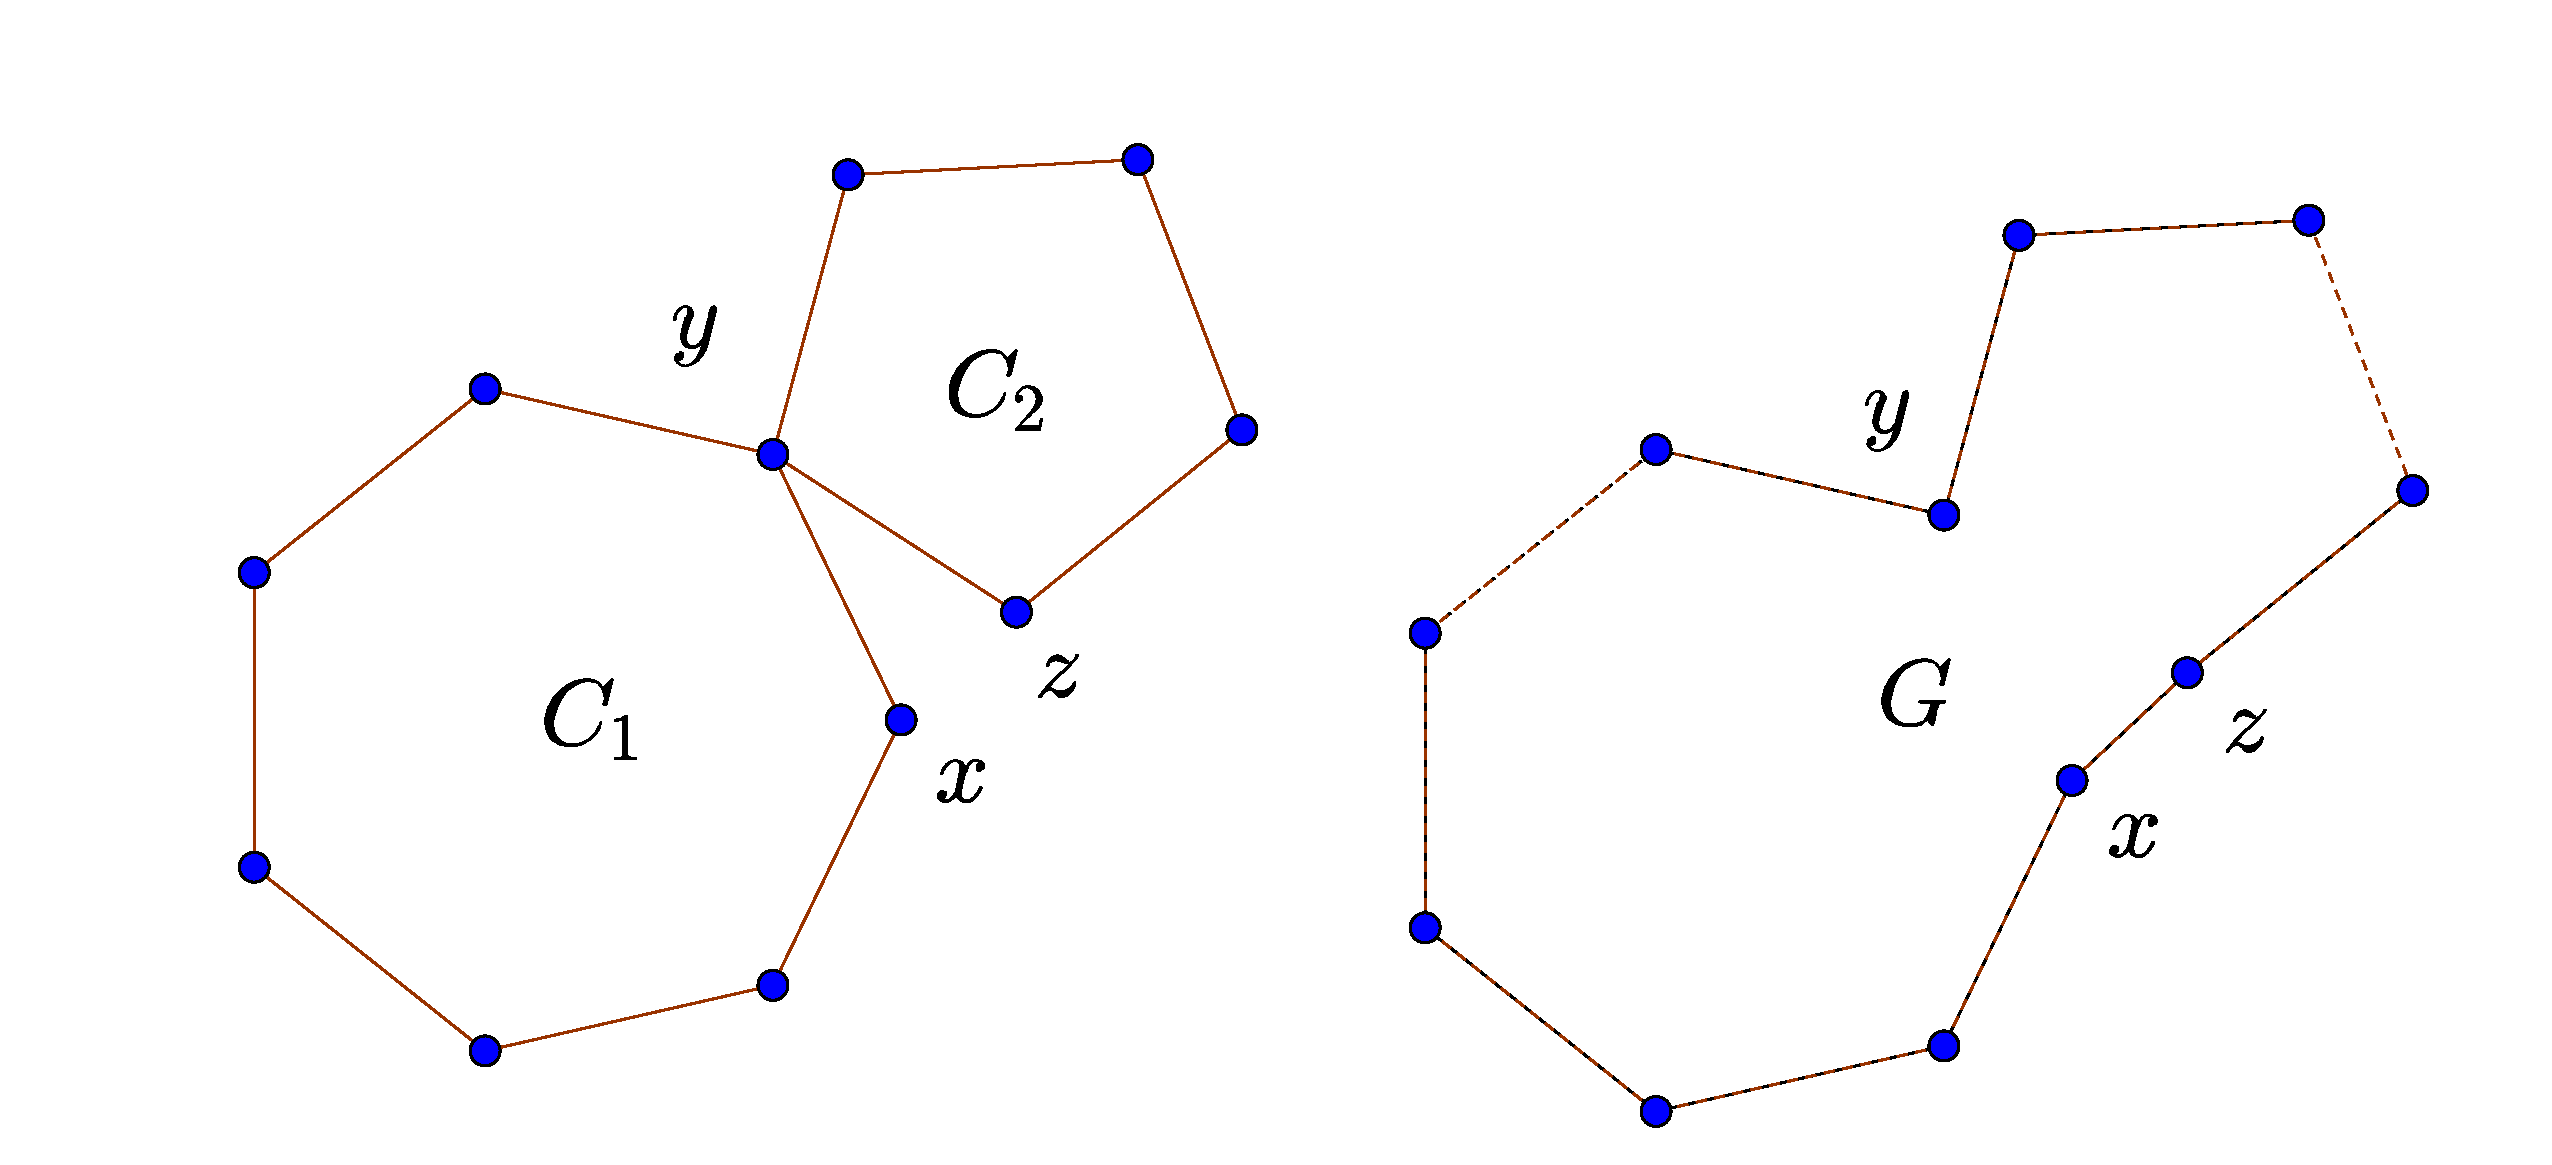
\includegraphics[scale=0.25]{oddcycles1.eps}
\end{figure*}

It remains to consider when $C_1$ and $C_2$ intersect multiple times, let $P$ and $Q$ be the longest path respectively of $C_1$ and $C_2$ with $y\in P\cap Q$ and where the only vertices that belong to $C_1\cap C_2$ are the endpoints of the paths.
Then $P\cup Q$ is a cycle that pass trough the edges $xy$ and $yz$, if the length of such cycle is even, by removing $xy,yz$ and adding $xz$ we get an odd cycle in $G$.

\begin{figure}[h]
\centering
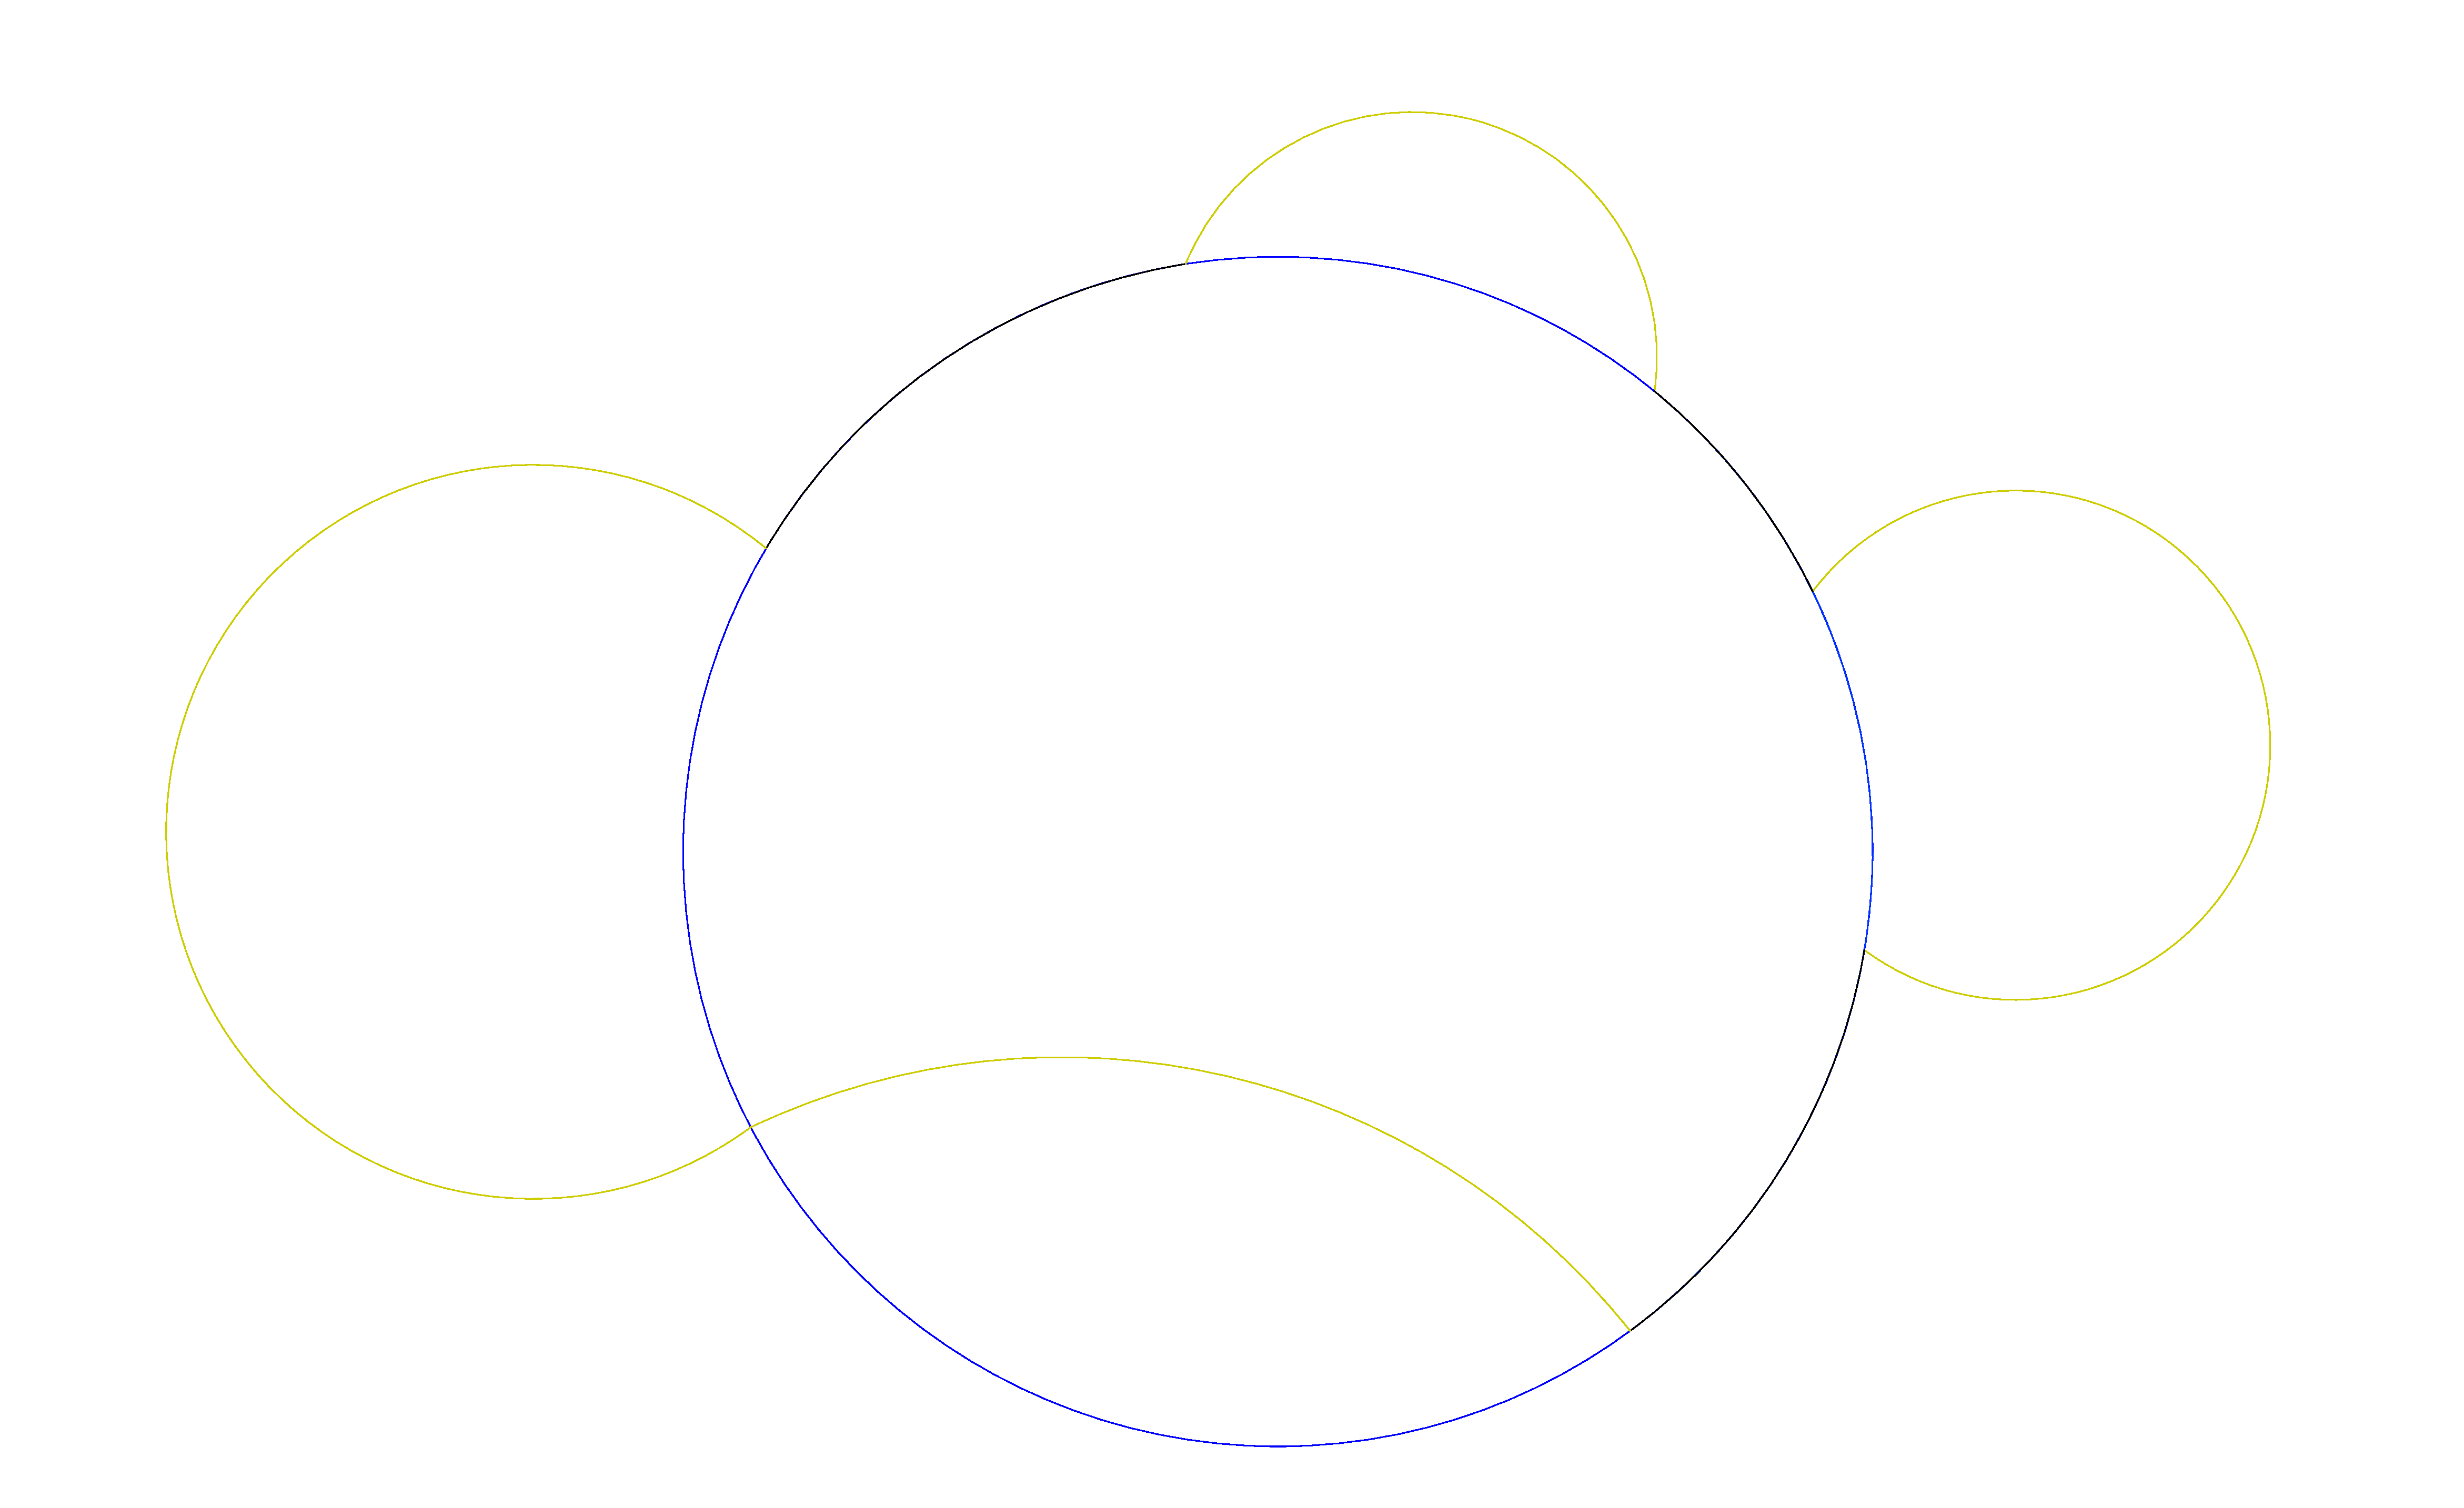
\includegraphics[scale=0.5]{oddcycles-interceptions.eps}
\caption{In blue $C_1 \backslash C_2 $, in green $C_2\backslash C_1 $ and in black the intersection }
\end{figure}
If $P\cup Q$ is an odd cycle, consider the remaining part which namely consists of $C_1\cap C_2$ and of $\tilde{C}_1,..,\tilde{C}_l$ cycles, then at at least one of them must be odd since $|P\cup Q|$ is odd and the following holds $$2n+1+2m+1-|P\cup Q| = \sum^l_{i=1} length(\tilde{C}_i) + 2\cdot |C_1\cap C_2|   $$
Finally, since $xy\in P$ and $yz\in Q$, such odd cycle is also in $G$. 

\QED

\newpage
\subsection*{Gallai-Hasse-Roy-Vitaver theorem}
\addcontentsline{toc}{subsection}{Gallai-Hasse-Roy-Vitaver theorem}

Another way to describe a proper colouring of a graph, is by introducing an order on the colours, indeed we may use the binary symbol $<$ and write $x<y$ to say "the vertex $x$ is coloured in a colour smaller than the one of the vertex $y$". We shall write $x\geq y $ instead of $\neg (x<y)$. The role of the formulas (\ref{color-prop1}), (\ref{color-prop2}) and (\ref{color-prop3}) is now played by 

\begin{gather}
x\geq x\\
x<y \e y<z \rightarrow x<z \\
( xy \in E \Rightarrow ) \qquad  x<y \o y<x\\
\bigvee_{i=0}^{n-1} x_i\geq x_{i+1}
\end{gather}
In the formalism of hyper resolution, for a given graph $G=(V,E)$ we consider the language $\mathscr{L}=\{\geq\}\cup V\cup E$, where $V\cup E$ are constants; the models are the $n$-colourable graphs that contains $G$ while the inference rules are
\begin{align*}
\prftree{\Gamma}{\Gamma \cup \{x\geq x\}}\qquad \qquad\qquad
& \qquad\prftree{\Gamma\cup\{x\geq y\}}{ \Sigma\cup\{y\geq z\} }{\Gamma\cup\Sigma\cup\{x\geq z\}} \\
\,&\,\\
\prftree[l]{$\quad xy \in E $}{\Gamma \cup \{ x\geq y \}}{\Sigma \cup \{ y\geq x \}}
{ \Gamma\cup\Sigma} \qquad &\qquad \prftree{\Gamma}
{\Gamma\cup\{x_0\geq x_1 ,..., x_{n-1}\geq x_n \}}
\end{align*}
The advantage of these rules respect the previous approach can be seen in the last rule, indeed now to describe a $n$-colouring it's enough to have an axiom that introduces $n-1$ literals while with (\ref{color-prop3}) we must involve $n(n+1)/2$ vertices for each instance.


Now, fix a simple graph $G$ and an orientation $D$ of $G$, we want to describe the property of Vitaver theorem "The directed paths in $D$ are not longer than $\ell (D)$" where $\ell (D)$ is defined to be the length of the longest directed path in $D$, maintaining the same notation as in Theorem \ref{vitaver}. To formalize such property we introduce the binary relation symbol \pred which is defined on pairs of vertices and which indicates the existence of a directed path from one vertex to the other
$$ x\pred y \Leftrightarrow \textrm{There is path from } x\textrm{ to } y $$
Since every arc can be seen as a path of length one, if there is an edge $xy$ in the underlying graph $G=(V,E)$ of $D$, then it's necessary  to have
\begin{equation}\label{pred1}
xy\in E \Rightarrow  x\pred y \o y\pred x
\end{equation}
If the end of the path is the start of another path, there exists a path which is the concatenation of the two:
\begin{equation}\label{pred2}
x\pred y \e y\pred z \rightarrow x\pred z
\end{equation}
Also, requiring that $\ell (D)$ is the maximum length of a path is equivalent to ask that there are no path of length equal to $n=\ell (D)+1$, which amounts to ask for any set of $n+1$ vertices
$$ \neg(x_0\pred x_1 \e x_1 \pred x_2 \e ...\e x_{n-1}\pred x_n )$$
and if we denote $\neg (x\pred y)$ as $x \npred y$ 
\begin{equation}\label{pred3}
x_0\npred x_1 \o x_1\npred x_2 \o ...\o x_{n-1}\npred x_n
\end{equation}
Finally, we require $D$ to be an acyclic orientation of $G$, which amounts to say that for any vertex $x$ there is no path from $x$ to $x$, that is:
\begin{equation}\label{pred4}
x\npred x
\end{equation}

Thus if we consider the language  $\mathscr{L}=\{\npred\}\cup V\cup E$, the models are the acyclic orientation of a subgraph of $G$ and the rules of inference are
\begin{align*}
\prftree{\Gamma}{\Gamma \cup \{x\npred x\}}\qquad \qquad\qquad
& \qquad\prftree{\Gamma\cup\{x\npred y\}}{ \Sigma\cup\{y\npred z\} }{\Gamma\cup\Sigma\cup\{x\npred z\}} \\
\,&\,\\
\prftree[l]{$\quad xy \in E $}{\Gamma \cup \{ x\npred y \}}{\Sigma \cup \{ y\npred x \}}
{ \Gamma\cup\Sigma} \qquad &\qquad \prftree{\Gamma}
{\Gamma\cup\{x_0\npred x_1 ,..., x_{n-1}\npred x_n \}}
\end{align*}
Clearly the rules have the same shape of the ones given for $\geq$, we can therefore conclude that $\npred$ describes an $n$-coloring for $G$ where
$$n=1+\min\{\ell(D'), D' \textrm{ spanning acyclic digraph of an orientation } \textrm{ of }G\}$$
If we consider an orientation $D$ of $G$ and a spanning acyclic digraph $D'$ of $D$, we have $\ell (D') \leq \ell(D)$ whence 
$$n\leq 1+ \ell $$
where $\ell$ is  $\min\{\ell(D), D \textrm{ orientation of }G\}$ as in corollary \ref{cor-vitaver}.\\
Finally recalling that P ropositions \ref{prop-vitaver-easy} says that for some orientation $D$
$$\chi (G) \geq 1+ \ell (D)$$
we reach the same conclusion of Corollary \ref{cor-vitaver}, i.e. 
$$\chi (G) = 1+\ell$$

\newpage
\subsection*{$\mu_n$ graphs}
\addcontentsline{toc}{subsection}{$\mu_n$ graphs}

The $\mu_n$ graphs are a family of graphs defined by Matiyasevich \cite{mat-1} with the purpose to characterize $n$-colurable graphs, first of all we will define the $\mu_2$ graphs then I will discuss the Matiyasevich theorem and how it can be used to rephrase problem such as the four colour theorem.

\begin{definition}
$\mu_n-graph$Matiyasevich
\end{definition}
\begin{itemize}
\item[-] Every complete graph with $n+1$ vertices is a $\mu_n$-graph
\item[-] If $G=(V,E)$ and $G'=(V',E')$ are $\mu_n$-graphs and $a,b,c$ are distinct vertices such that
$$ a,b\in V \quad b,c\in V'  $$
and
$$ ab\in E, ab\notin E' \qquad  bc\in E', bc\notin E$$
Then the graph $G''=(V\cup V', E\cup E'\cup\{ac\} \setminus\{ab,bc\} )$ is a $\mu_n$-graph.
\end{itemize} 
To understand better how such graphs look like, it is convenient to explore the $\mu_2$ graphs
\begin{proposition}
The odd cycles are $\mu_2$ graphs
\end{proposition}
\noindent\textit{Proof:}\\
Since the $\mu_2$ graphs are defined by induction, the proof will proceed by induction on the number of vertices.
First, the 3-cycle is the complete graph with 3 vertices then it is $\mu_2$ by definition. Thus let $x_1...x_n$ be a cycle with $n$ odd, the cycles $x_1x_2x_3$ and $x_3x_4...x_n$ are of odd length and therefore by induction they are $\mu_2$, then the second point of the definition applies by taking 	$a=x_1$, $b=x_3$ and $c=x_n$, hence the original cycle is $\mu_2$
\QED

\noindent On the other hand, not all $\mu_2$ graphs are odd cycles, the following example shows a $\mu_2$ graph which is not a cycle and which can be built using the definition and starting by a 3-cycle and a 5-cycle 
\begin{figure*}[h]
\centering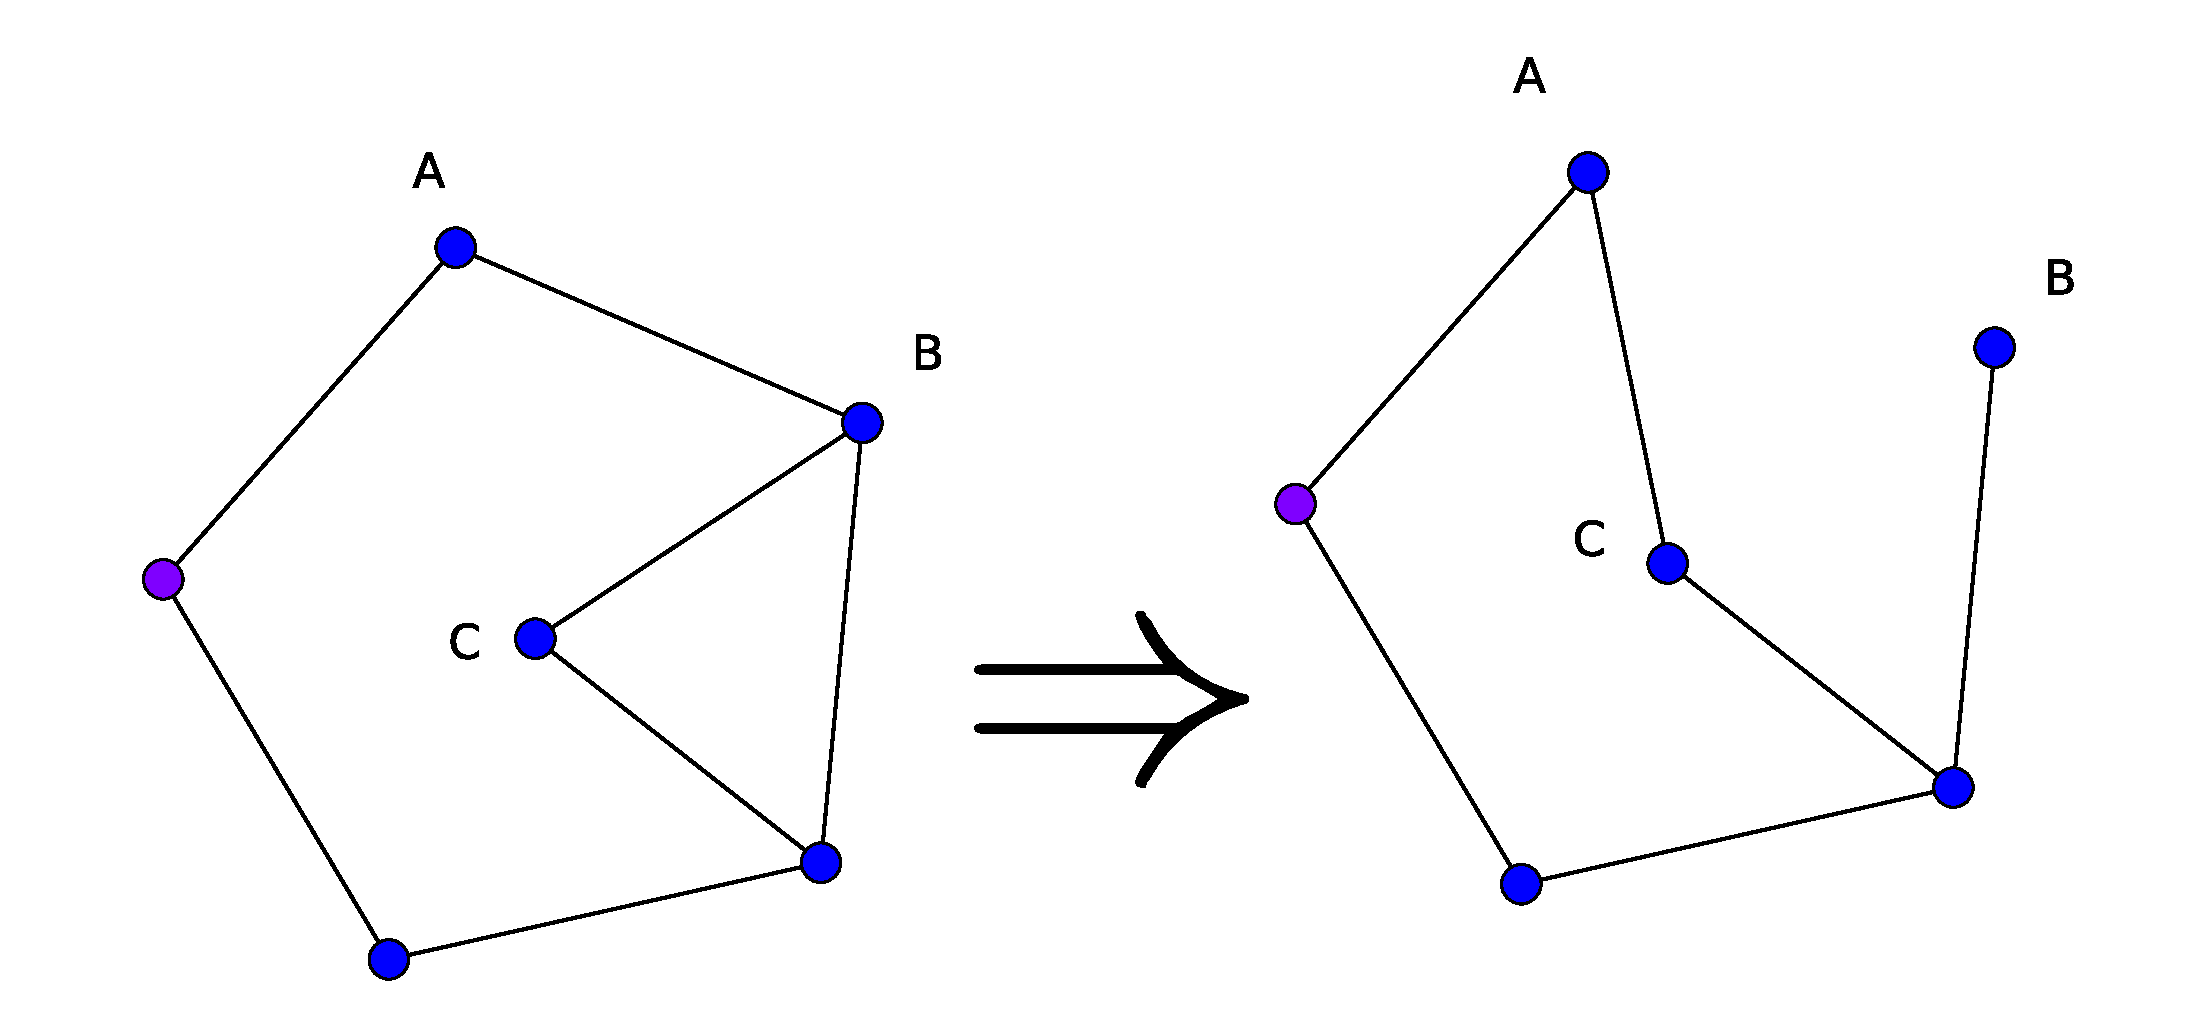
\includegraphics[scale=0.25]{mu2.eps}
\end{figure*}

\noindent They do not even need to be connected, indeed starting from these two $\mu_2$ graphs
\begin{figure*}[h]
\centering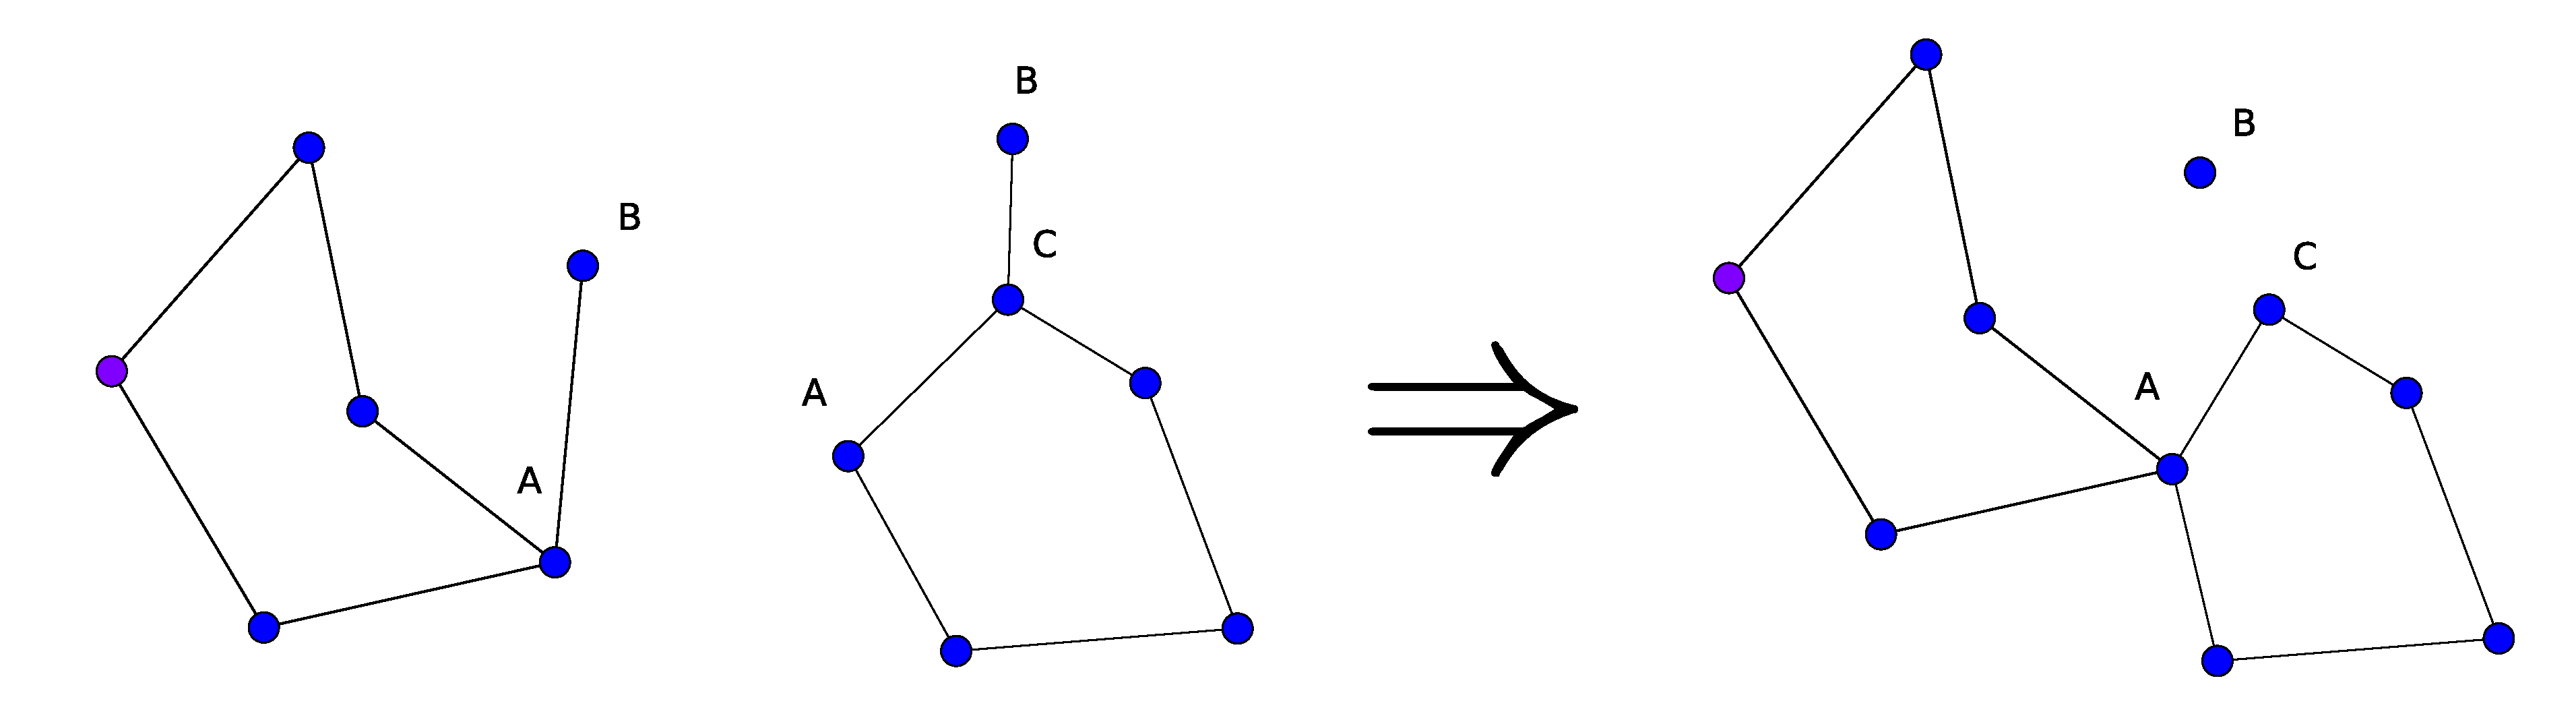
\includegraphics[scale=0.25]{mu2-con1.eps}
\end{figure*}

\noindent we can apply the definition to make the following construction that produces a non-connected $\mu_2$ graph 
\begin{figure*}[h]
\centering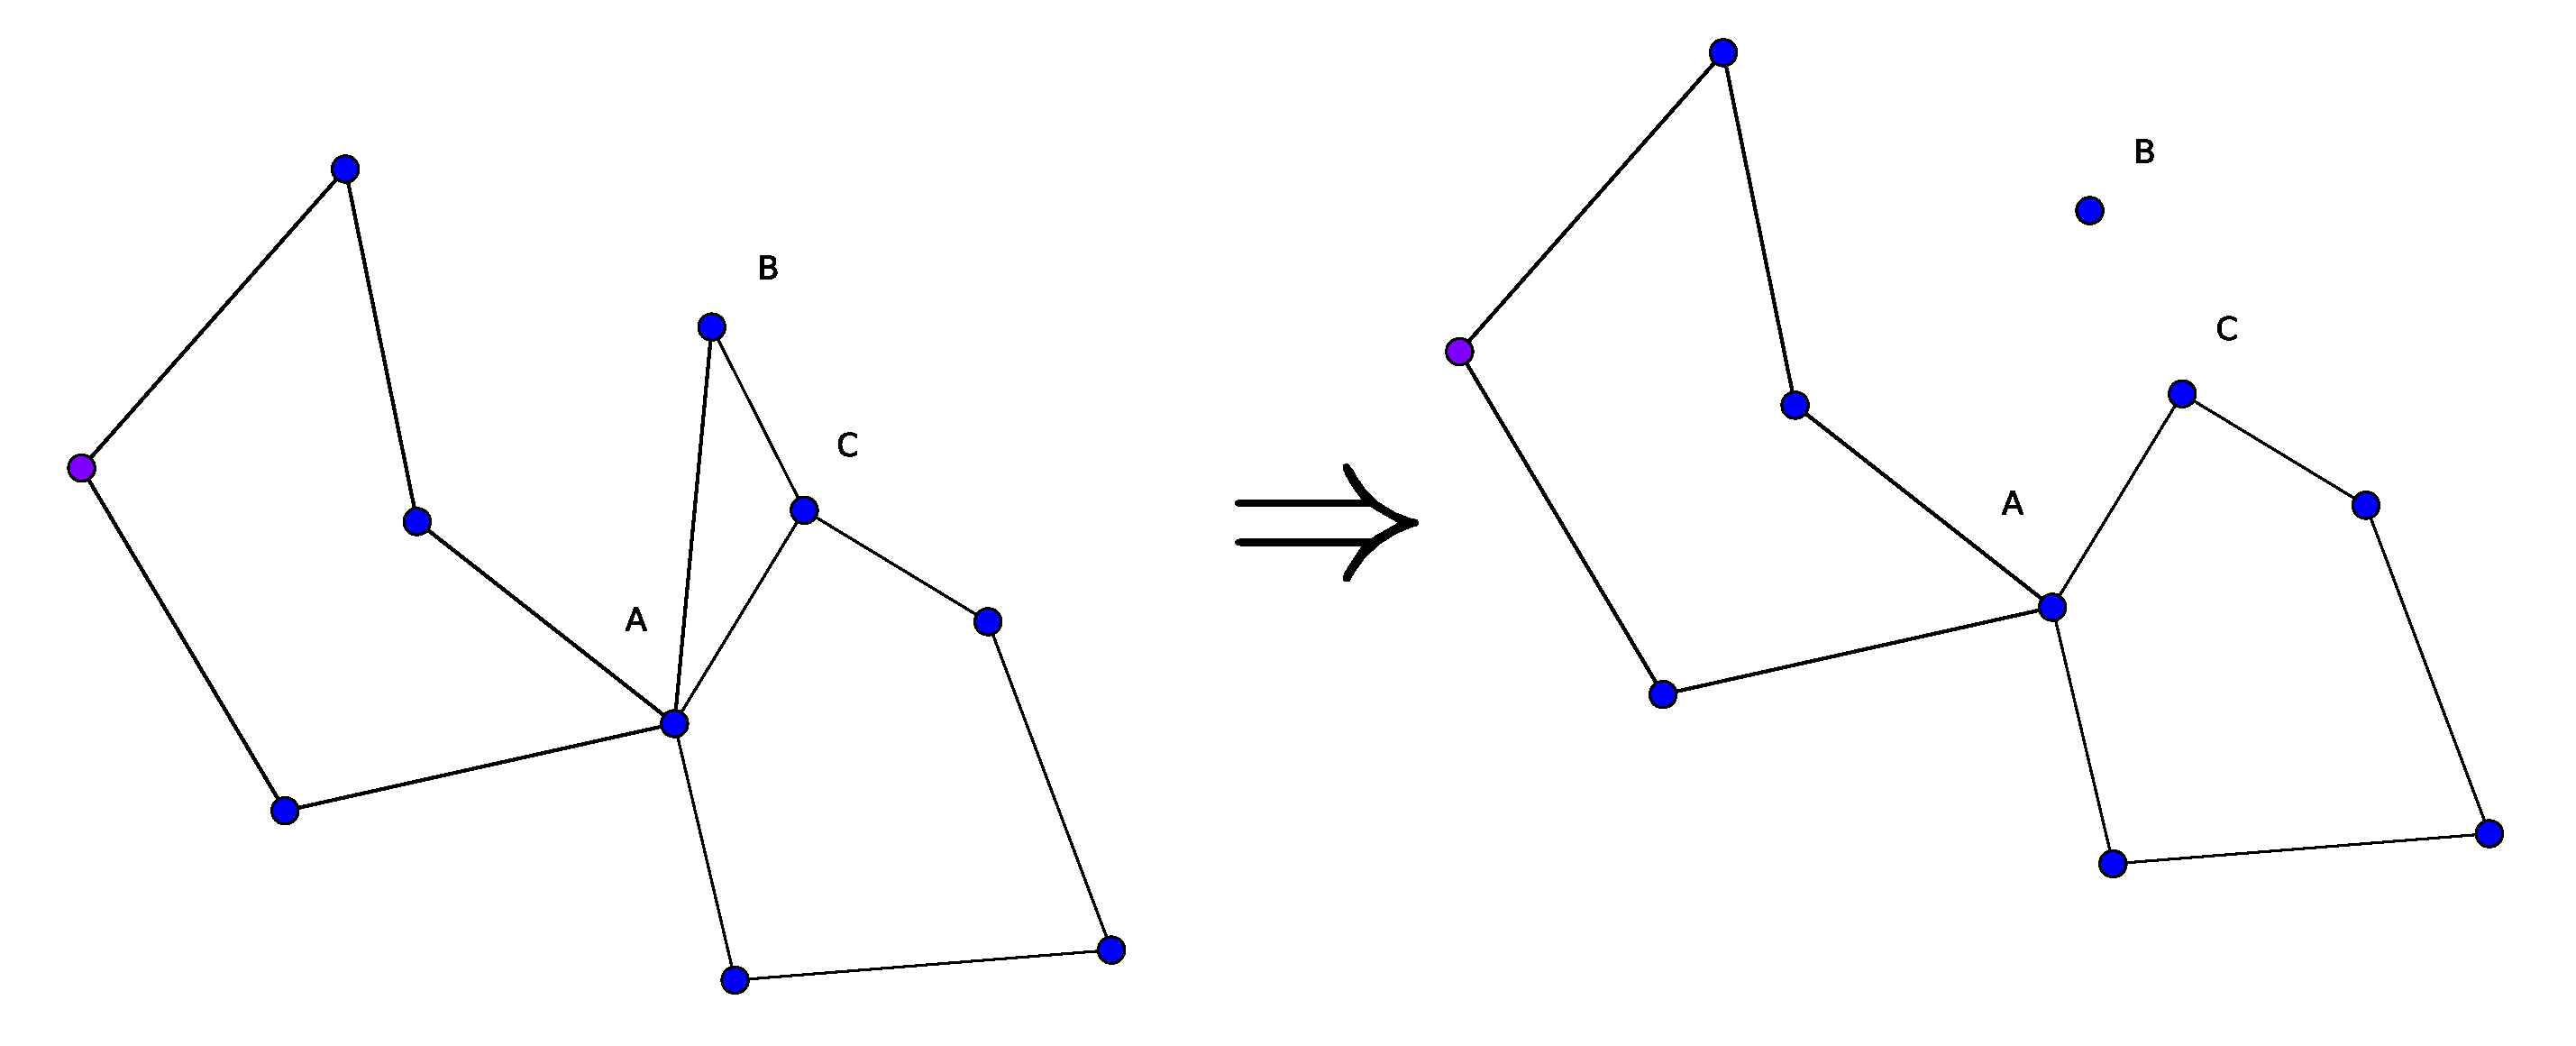
\includegraphics[scale=0.25]{mu2-con2.eps}
\end{figure*}

\newpage
The result obtained Matiyasevich gives a characterization of $n$-colourable graphs, the proof is 

\newpage
\phantomsection
\addcontentsline{toc}{chapter}{Bibliography}
\begin{thebibliography}{9}
\bibitem{lifschitz} 
Vladimir Lifschitz.
\textit{Semantical completeness theorems in logic and algebra.} 
American Mathematical Society, Vol. 79 No. 1, May 1980, Pages: 89-96 
 
\bibitem{robinson} 
John Alan Robinson.  
\textit{A Machine-oriented logic based on the resolution principle.} 
Journal of the association for computing machinery, Vol. 12 No. 1, January 1965, Pages:23-41

\bibitem{rob}
John Alan Robinson.  
\textit{Automatic deduction with hyperresolution} 
Int. J. Comp. Math. , Vol. 1, 1965, Pages:227-234
 
\bibitem{robinson-general} 
John Alan Robinson.  
\textit{The generalized resolution principle.} 
??????

\bibitem{mat-1} 
Jurij Vladimirovi\v{c} Matijasevi\v{c}.
\textit{Mathematical approach to proving theorems of discrete mathematics.} 
Seminar in mathematics, Steklov mathematical institute, Leningrad, 1975, Pages:31-48

\bibitem{mat-2}
Jurij Vladimirovi\v{c} Matijasevi\v{c}.
\textit{Application of the methods of the theory of logical derivation to graph- theory.} Mathematicheskie Zametki, Vol. 12 No. 6, December 1972, Pages: 781-790
 
\bibitem{gallier} Jean H. Gallier. \textit{Logic for Computer Science, Foundations of automatic theorem proving }

\bibitem{diestel} Reinhard Diestel. \textit{Graph Theory}

\bibitem{chrom} Gary Chartrand, Ping Zhang. \textit{Chromatic Graph Theory}

\bibitem{vitaver} L.M. Vitaver \textit{Determination of minimal colorings of graph vertices with the aid of boolean powers of the adjacency matrix.} Dokl. Akad. Nauk SSSR, 147 No 4., 1962, Pages: 758-759

\bibitem{hasse} Maria Hasse \textit{Zur algebraischen Begrundung der Graphentheorie. I} Mathematische Nachrichten (in German), 1965, Pages: 275–290,

\bibitem{roy}B. Roy, Nombre chromatique et plus longs chemins d’un graph. Rev AFIRO
1 (1967) 127-132.

\bibitem{gallai}T. Gallai, \textit{On directed paths and circuits}. In: Theory of Graphs; Proceedings of the Colloquium held at Tihany, Hungary, 1969 (P. Erd ̋s and G. Katona,eds). Academic Press, New York (1969) 115-118.





\end{thebibliography}


\end{document}
